% !TEX TS-program = pdflatex
% !TEX encoding = UTF-8 Unicode

\documentclass[11pt]{article} % use larger type; default would be 10pt

\usepackage[utf8]{inputenc} % set input encoding (not needed with XeLaTeX)

%%% PAGE DIMENSIONS
\usepackage{geometry} % to change the page dimensions
\geometry{a4paper} % or letterpaper (US) or a5paper or....


%%%%%% PACKAGES%%%%%%%%%%%%%%%%%%

%%Less commonly used packages are commented
\usepackage{graphicx} % support the \includegraphics command and options
\usepackage{siunitx} %Add nice SI units, also nice scientific notation
\usepackage{amssymb} %ams packages add many math symbols and functions
\usepackage{amsmath}
\usepackage{amsthm}
\usepackage{hyperref}
%\usepackage{biblatex}


%\usepackage{indentfirst} %Indents first line after section heading
%\usepackage{array} % for better arrays (eg matrices) in maths
%\usepackage{float} %Add options for tricking figures into behaving
%\usepackage{circuitikz} %Add circuit diagrams
\usepackage{tikz} %Add inline vector graphics drawing (included in circuitikz)
%\usepackage{chemfig} %Add chemical structure drawing
%\usepackage{verbatim} % adds environment for commenting out blocks of text & for better verbatim
%\usepackage{subfig} % make it possible to include more than one captioned figure/table in a single float
\usepackage{subcaption}
\usepackage{multicol}
%\usepackage{booktabs} % for much better looking tables
%\usepackage{paralist} % very flexible & customisable lists (eg. enumerate/itemize, etc.)
%\usepackage{qtree}  % Add tree diagrams
%\usepackage{listings} % for nice code blocks
%\usepackage{makeidx} % for index stuff 
%\makeindex          % should be included if using index

%%%%%%%%%%%%%%%%%%%%%%%%%%%%%%%%%%%%%%%%

%%%%%%Code Block Style Definition%%%%%%%

%%%Only compiled if listings included%%%

\ifdefined\lstdefinestyle{}{}
\usepackage{xcolor}

\definecolor{codeback}{RGB}{220,223,242}
\definecolor{codekeyword}{RGB}{10,199,17}
\definecolor{codestring}{RGB}{223,40,40}
\definecolor{codecomment}{RGB}{13,68,201}
\definecolor{altcodekeyword}{RGB}{226,127,58}

\lstdefinestyle{AICode}{
	basicstyle = \ttfamily,
	backgroundcolor = \color{codeback},
	keywordstyle = \color{codekeyword},
	numberstyle = \scriptsize\color{gray},
	stringstyle = \color{codestring},
	commentstyle = \color{codecomment},
	tabsize = 4,
	numbers = left
}

\lstset{style=AICode}

\fi


%%%%%%%%%%%%%%%%%%%%%%%%%%%%%%%%%%%%%%%%%

%%% HEADERS & FOOTERS
\usepackage{fancyhdr} % This should be set AFTER setting up the page geometry
\pagestyle{fancy} % options: empty , plain , fancy
\renewcommand{\headrulewidth}{0pt} % customise the layout...
\lhead{}\chead{}\rhead{}
\lfoot{}\cfoot{\thepage}\rfoot{}


\numberwithin{equation}{section}  %make equation numbers be (section.eqn number)

%%%%%%Some QOL shortcuts (mostly math symbols)%%%%%%%%%%%%%%%
\newcommand{\R}{\mathbb{R}}       %quick real number symbol
\newcommand{\Z}{\mathbb{Z}}		  %Integers
\newcommand{\Q}{\mathbb{Q}}	      %Rationals
\newcommand{\C}{\mathbb{C}}       %Complex Numbers
\newcommand{\N}{\mathbb{N}}       %Naturals

\newcommand{\p}{\partial}              %partial derivative
\newcommand{\curl}{\text{curl}}      %divergence and curl
\newcommand{\dv}{\text{div}}
\newcommand{\tb}[1]{\textbf{#1}}  %quicker bold and italic text
\newcommand{\ti}[1]{\textit{#1}}

\renewcommand{\thesection}{\Roman{section}}

\newcommand{\splitpage}[2]{  %Temporarily split page into two
\noindent
\begin{minipage}{.5\textwidth}
#1
\end{minipage}%
\begin{minipage}{.5\textwidth}
#2
\end{minipage}}

%%%%%%%%%%%%%%%%%%%%%%%%%%%%%%%%%%%%%%%%%%


%%%%%%'Variable' definitions to make fill-in-the-blank type info easier%%%%%%%
\newcommand{\prof}{PROFFESSOR_NAME_HERE}
\newcommand{\sem}{SEMESTER(SEASON)_HERE}
\newcommand{\yr}{YEAR_TAKEN_HERE}
\newcommand{\deptnum}{DEPARTMENT_AND_NUMBER_HERE}
\newcommand{\coursetitle}{COURSE_TITLE_HERE}

%%%%%%%%%%%%%%%%%%%%%%%%%%%%%%%%%%%%%%%%%%


%%%%%%%%%%%%%Title%%%%%%%%%%%%%
\title{Results for Learned Evolution Function on the Bloch Sphere}
\date{} % Activate to display a given date or no date (if empty),
         % otherwise the current date is printed 

%%%%%%%%%%%%%%%%%%%%%%%%%%%%


%%%%%%%%%%%%%%%%%%%%%%%%%%%
%%%%%%%START OF DOCUMENT%%%%%%%%%
%%%%%%%%%%%%%%%%%%%%%%%%%%%

\begin{document}
\maketitle


%%%%%%%End of front matter%%%%%%%%%%

\begin{multicols}{2}

\section{Methodology}
The nonlinear network is a dense neural network, where each layer is activated by SeLUs and optimized with the Adam optimizer.  There are six layers, with 64, 256, 512, 512, 256, and 64 neurons respectively.  Each model is trained for 250 epochs with a learning rate of $10^{-3}$ followed by another 250 epochs with a learning rate of $10^{-4}$.  The nonlinear network is put between the encoder and decoder of an autoencoder network which has already been trained on points on the Bloch sphere and is frozen.  

The training is done by putting points on the Bloch sphere through the entire network and then comparing the output to the result from the Schr\"odinger equation.  The loss used is the L2 distance between the output point and the point given by the Schr\"odinger equation.  Initial conditions were sampled as a normal distribution and evolved on the Bloch sphere using the constant Hamiltonian
\[\mathcal{H} = \begin{pmatrix}
	0.5567+0i & 0.9560+0.7846i\\
	0.9560-0.7846i & 0.0873+0i
\end{pmatrix}\]

We set aside 10\% of the available evolutions for validation.   



\section{Results}
We have measured most of our results as functions of timestep, evolution time, and number of initial conditions.

\subsection{Linear Recovery}
Our entire end-to-end network (encoding$\to$ evolution$\to$ decoding) is ideally equivalent to the Schr\"odinger equation, and thus should be linear.  Then we should have

\begin{multline}\label{linear_eqn}
\phi^{-1}\circ F^t\circ \phi(\alpha(v+w))=\\ 
\alpha(\phi^{-1}\circ F^t\circ \phi(v) + \phi^{-1}\circ F^t\circ \phi(w)).
\end{multline}


In order to test this, we select points $v$ and $w$ in our training set such that $\alpha(v+w)$ is approximately in our dataset as well (there is some $\widetilde{v+w}$ such that $\|\alpha(v+w)-\widetilde{v+w}\|_2 < \epsilon$).  $\alpha$ is selected such that $v+w$ has a norm of 1.  Since it is in the training set and thus a point on the Bloch sphere, $\widetilde{v+w}$ will have this $\alpha$ factor built in, so in code the $\alpha$ only appears on the right hand side of the equation.

We select the test points to be in our training set in order to ensure that any difference between the two sides of the equation is due to lost linearity, rather than poor predictions on the part of one of the models.

\end{multicols}

\begin{figure}
	\centering
	
	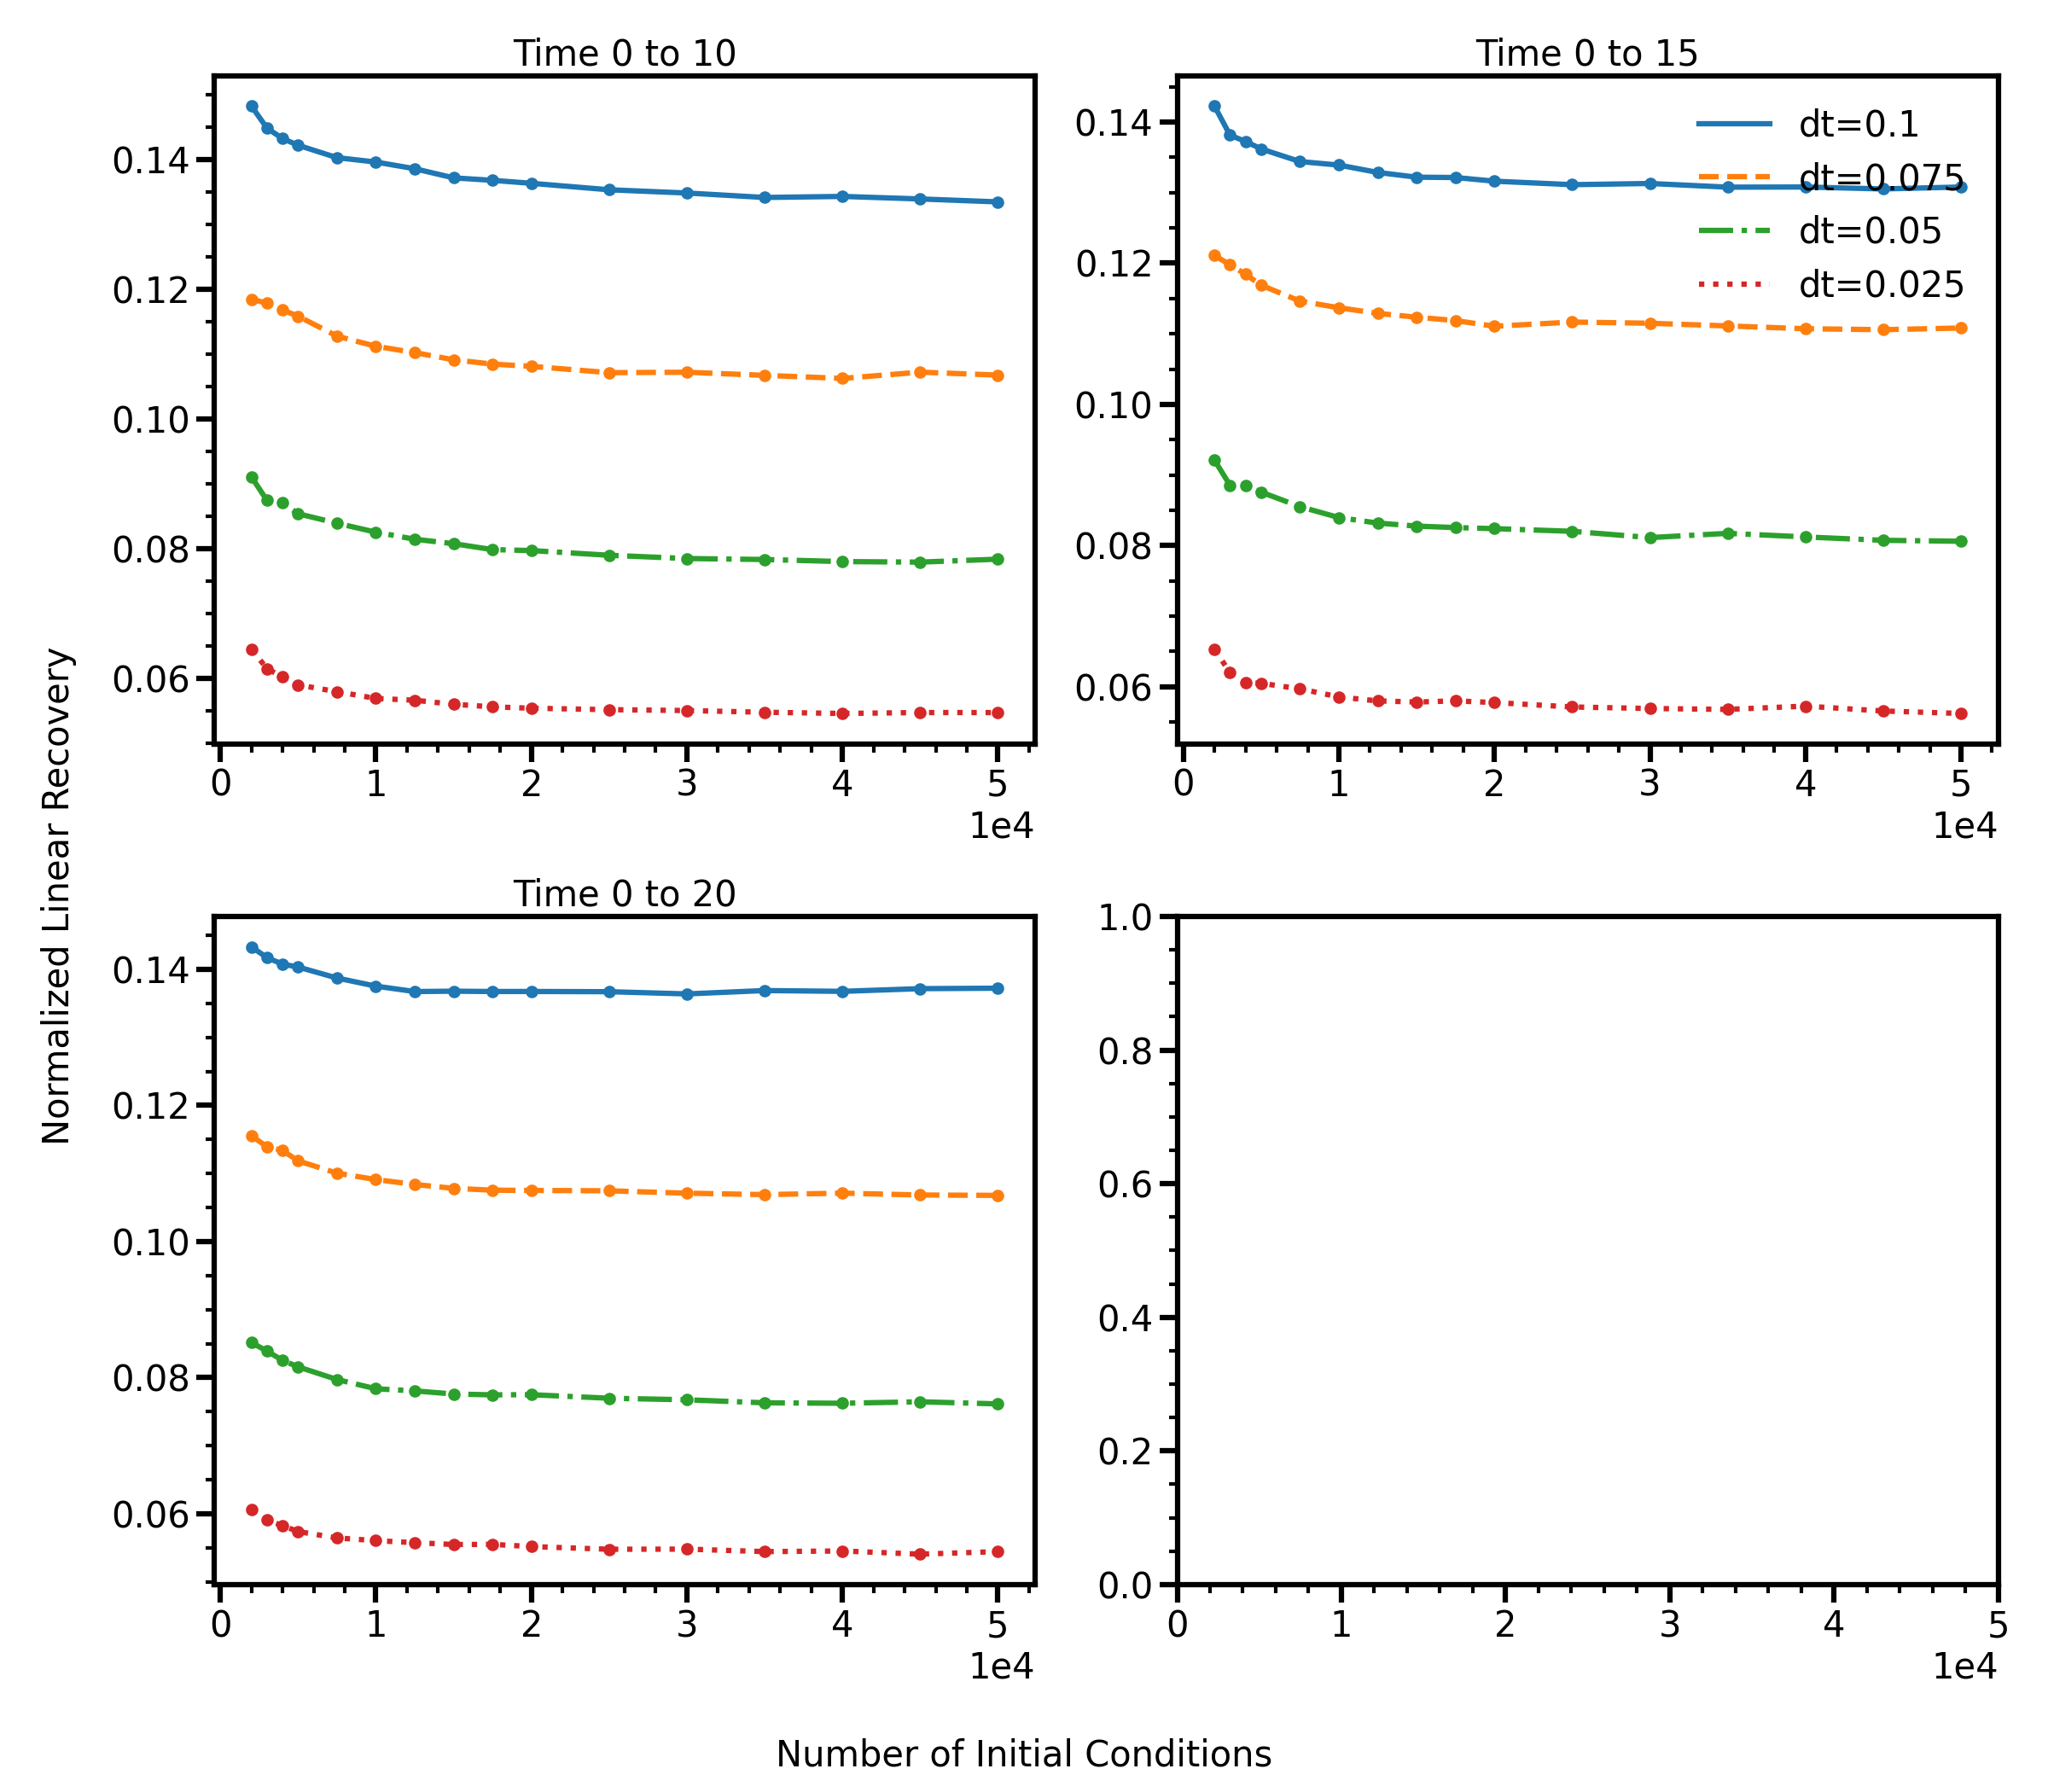
\includegraphics[width=\linewidth]{figures/norm_linear_recovery}
	
	\caption{Linear recovery after timestep normalization.}\label{norm_linear_recovery}
\end{figure}



\begin{figure}
	\centering
	
	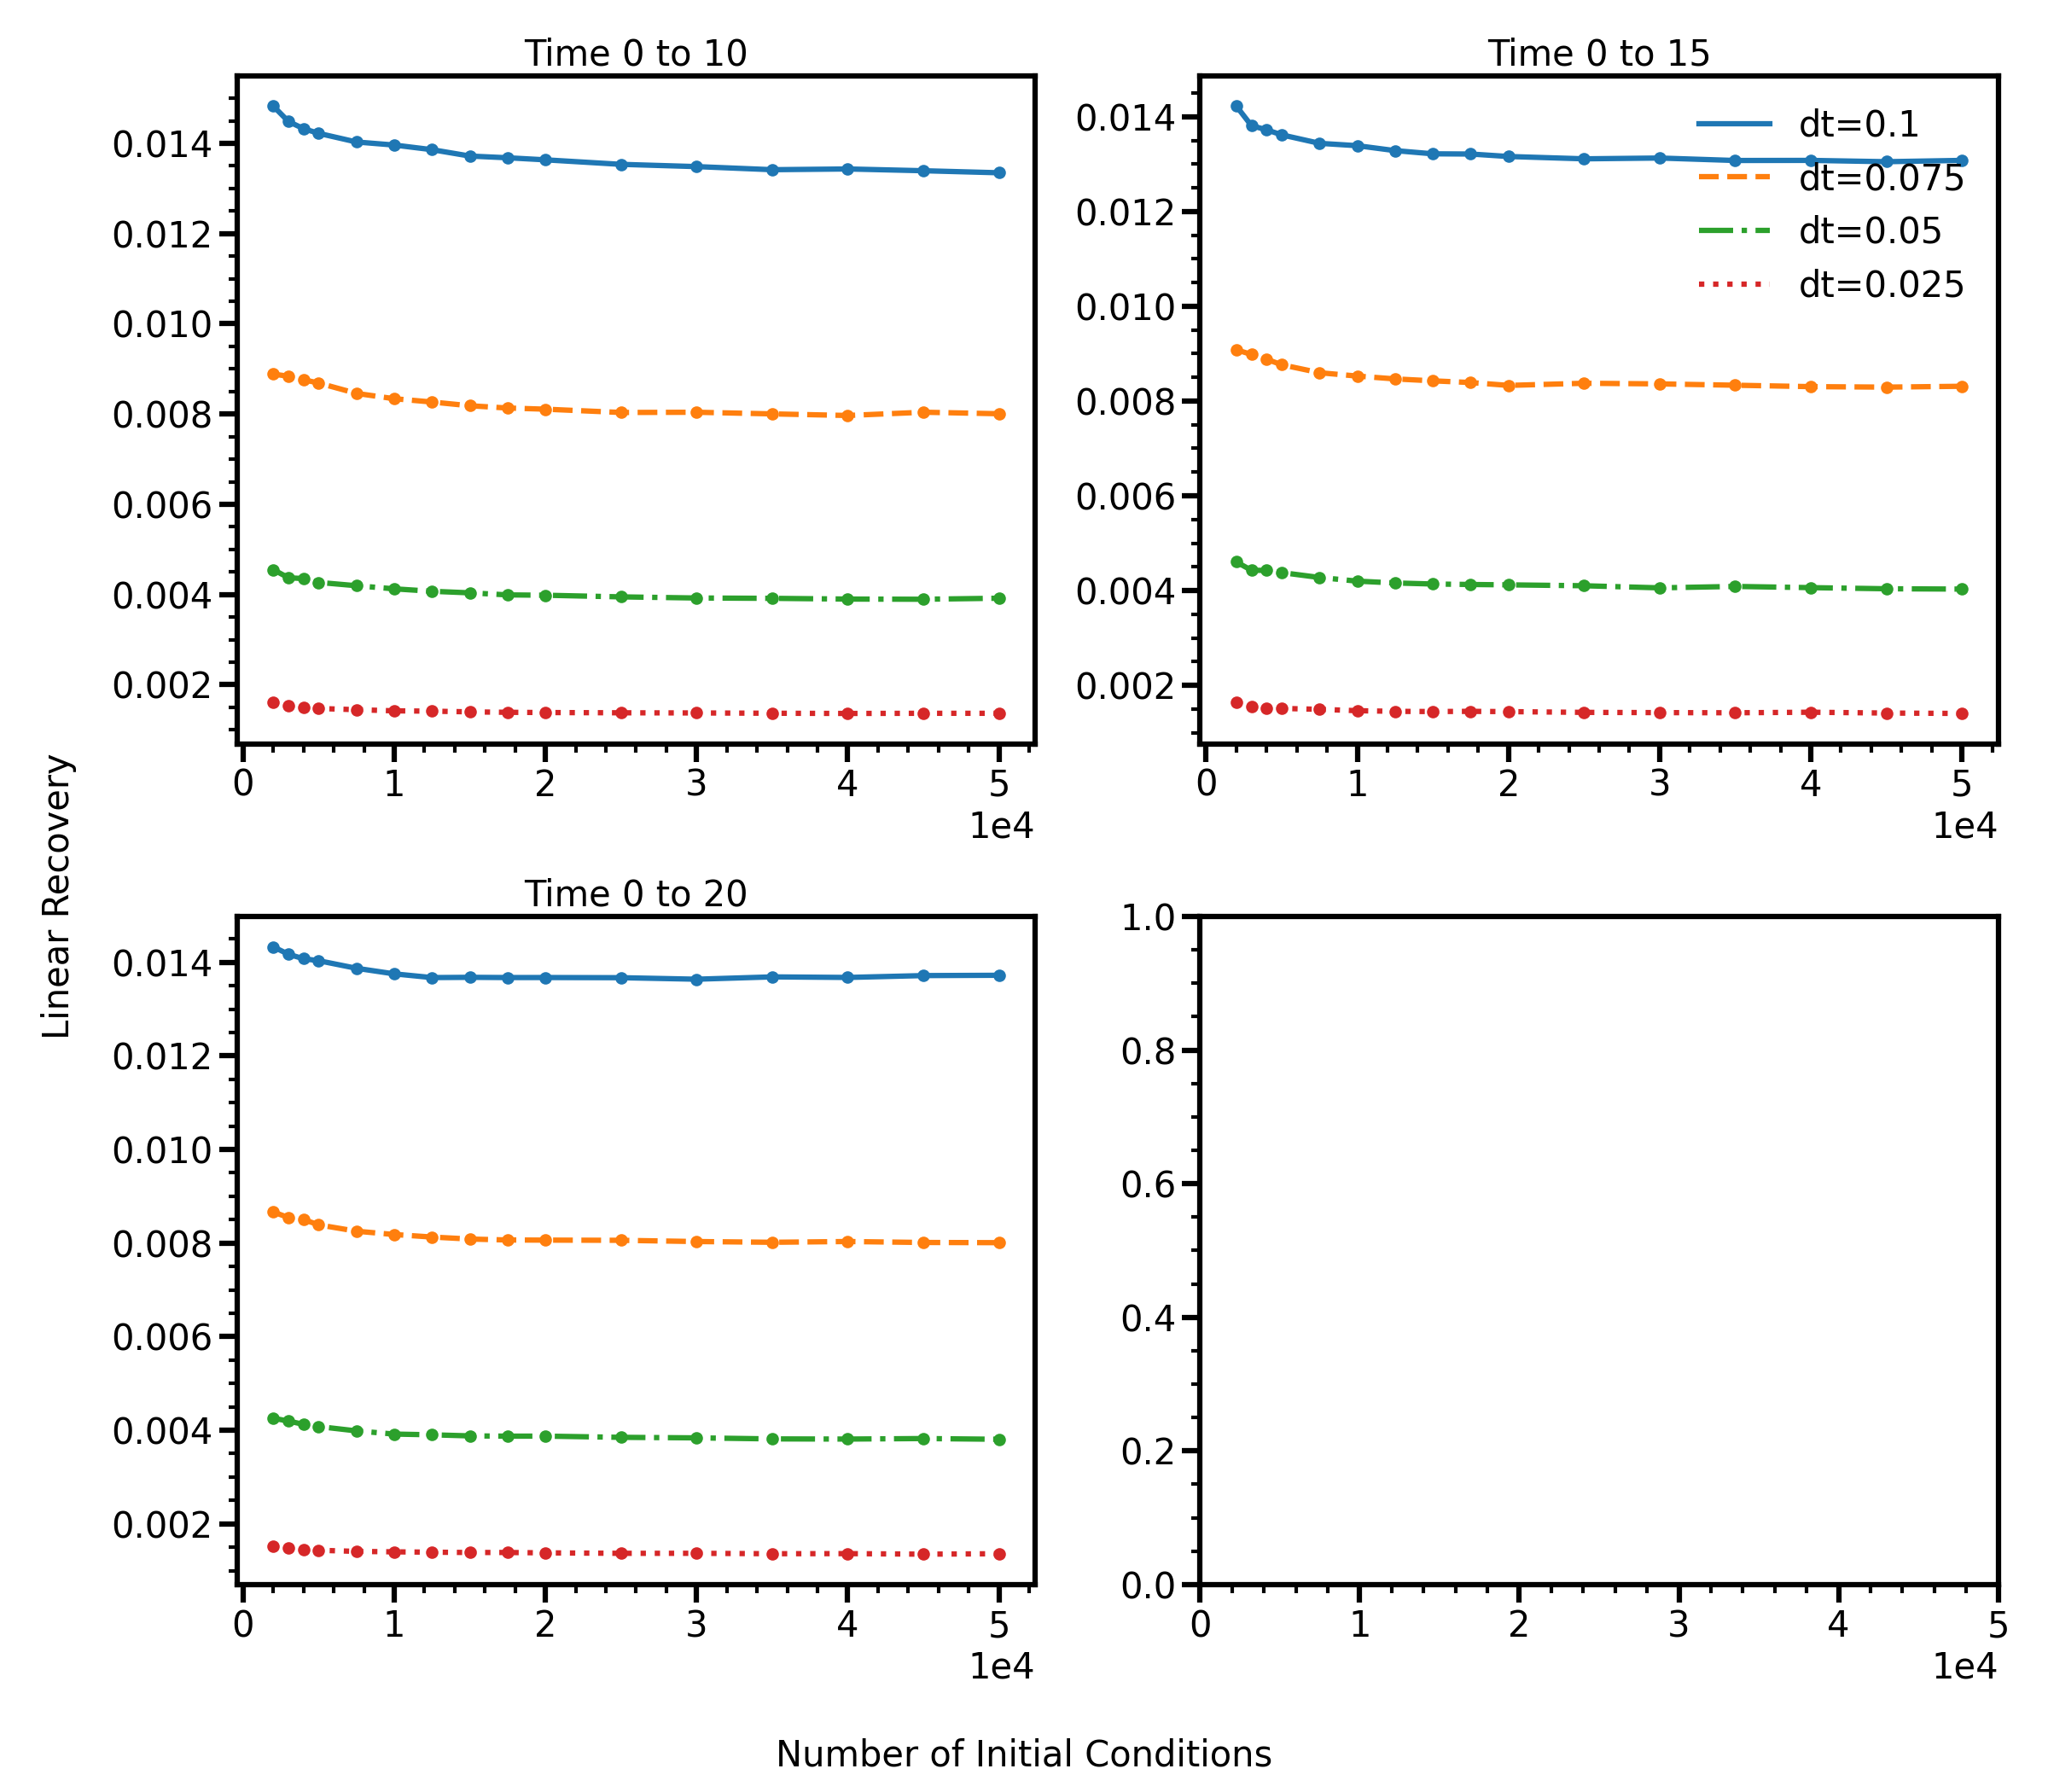
\includegraphics[width=\linewidth]{figures/nonnorm_linear_recovery}
	
	\caption{Linear recovery before timestep normalization.}\label{nonnorm_linear_recovery}
\end{figure}


\begin{multicols}{2}

Before normalization, linearity is recovered out to two decimal places, which is as far as the model is accurate to (see \ref{Accuracy}, particularly figure \ref{nonnorm_val_loss}).  We note that the linear recovery is roughly constant across evolution time and has only a light dependence on the number of initial conditions.  

Looking instead to the linear recovery plotted with a constant timestep as in figures \ref{norm_linear_recovery_evolve_time} and \ref{nonnorm_linear_recovery_evolve_time}, we can more easily see how the linear recovery changes with respect to the evolution time.  Note that the differences in the evolution time primarily happen at the third decimal, beyond our model's maximum range of accuracy, hence some of the strange behavior.


\subsection{Nonlinearity}
By our hypothesis, the learned evolution function function should be nonlinear.  To measure this, we find the L2 distance between $F^t(\phi(v)+\phi(w))$ and $F^t(\phi(v))+F^t(\phi(w))$.  Unlike when checking for linearity, when checking for nonlinearity we must make sure that $\phi(v),\phi(w)$, and $\phi(v)+\phi(w)$ are all in the (compressed) dataset.  This is due to checking for nonlinearity only in the compressed space which $F^t$ acts in (we already know that $\phi$ and $\phi^{-1}$ are nonlinear).  The larger our nonlinearity value is, the more nonlinear our function.

\end{multicols}

\begin{figure}
	\centering
	
	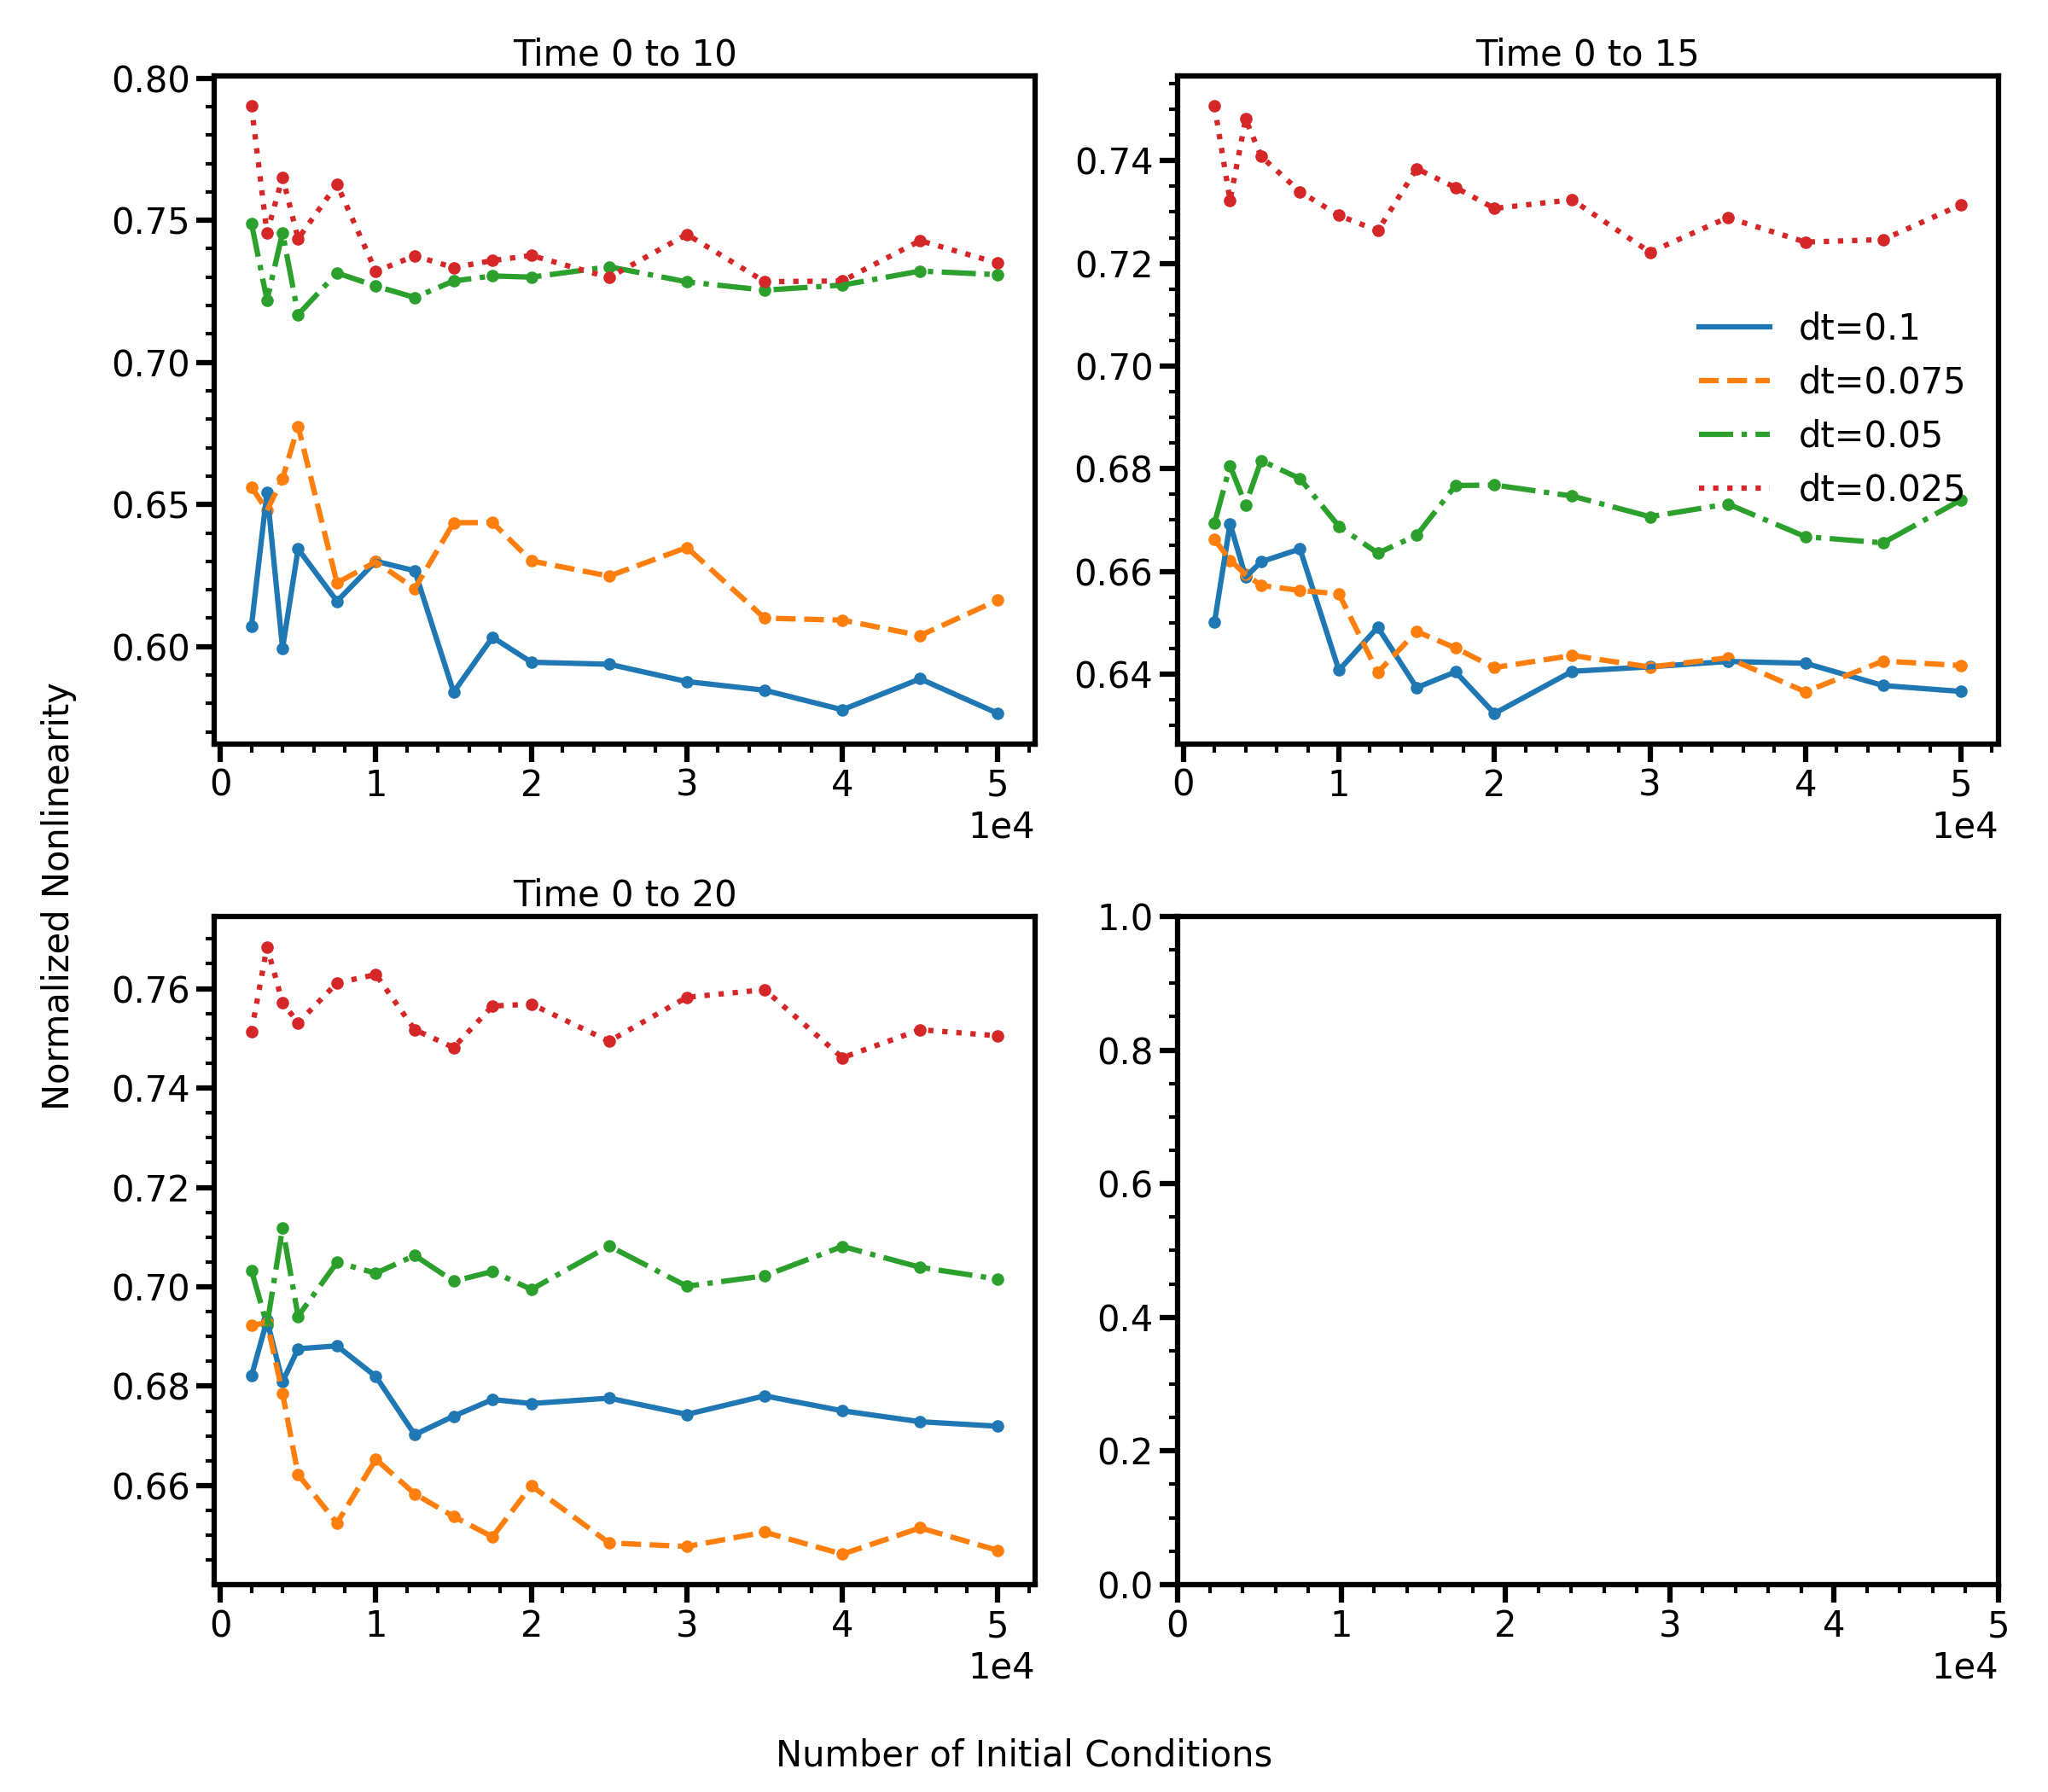
\includegraphics[width=\linewidth]{figures/norm_nonlinearity}
	
	\caption{Nonlinearities after normalization.  }\label{norm_nonlniear}
\end{figure}


\begin{figure}
	\centering
	
	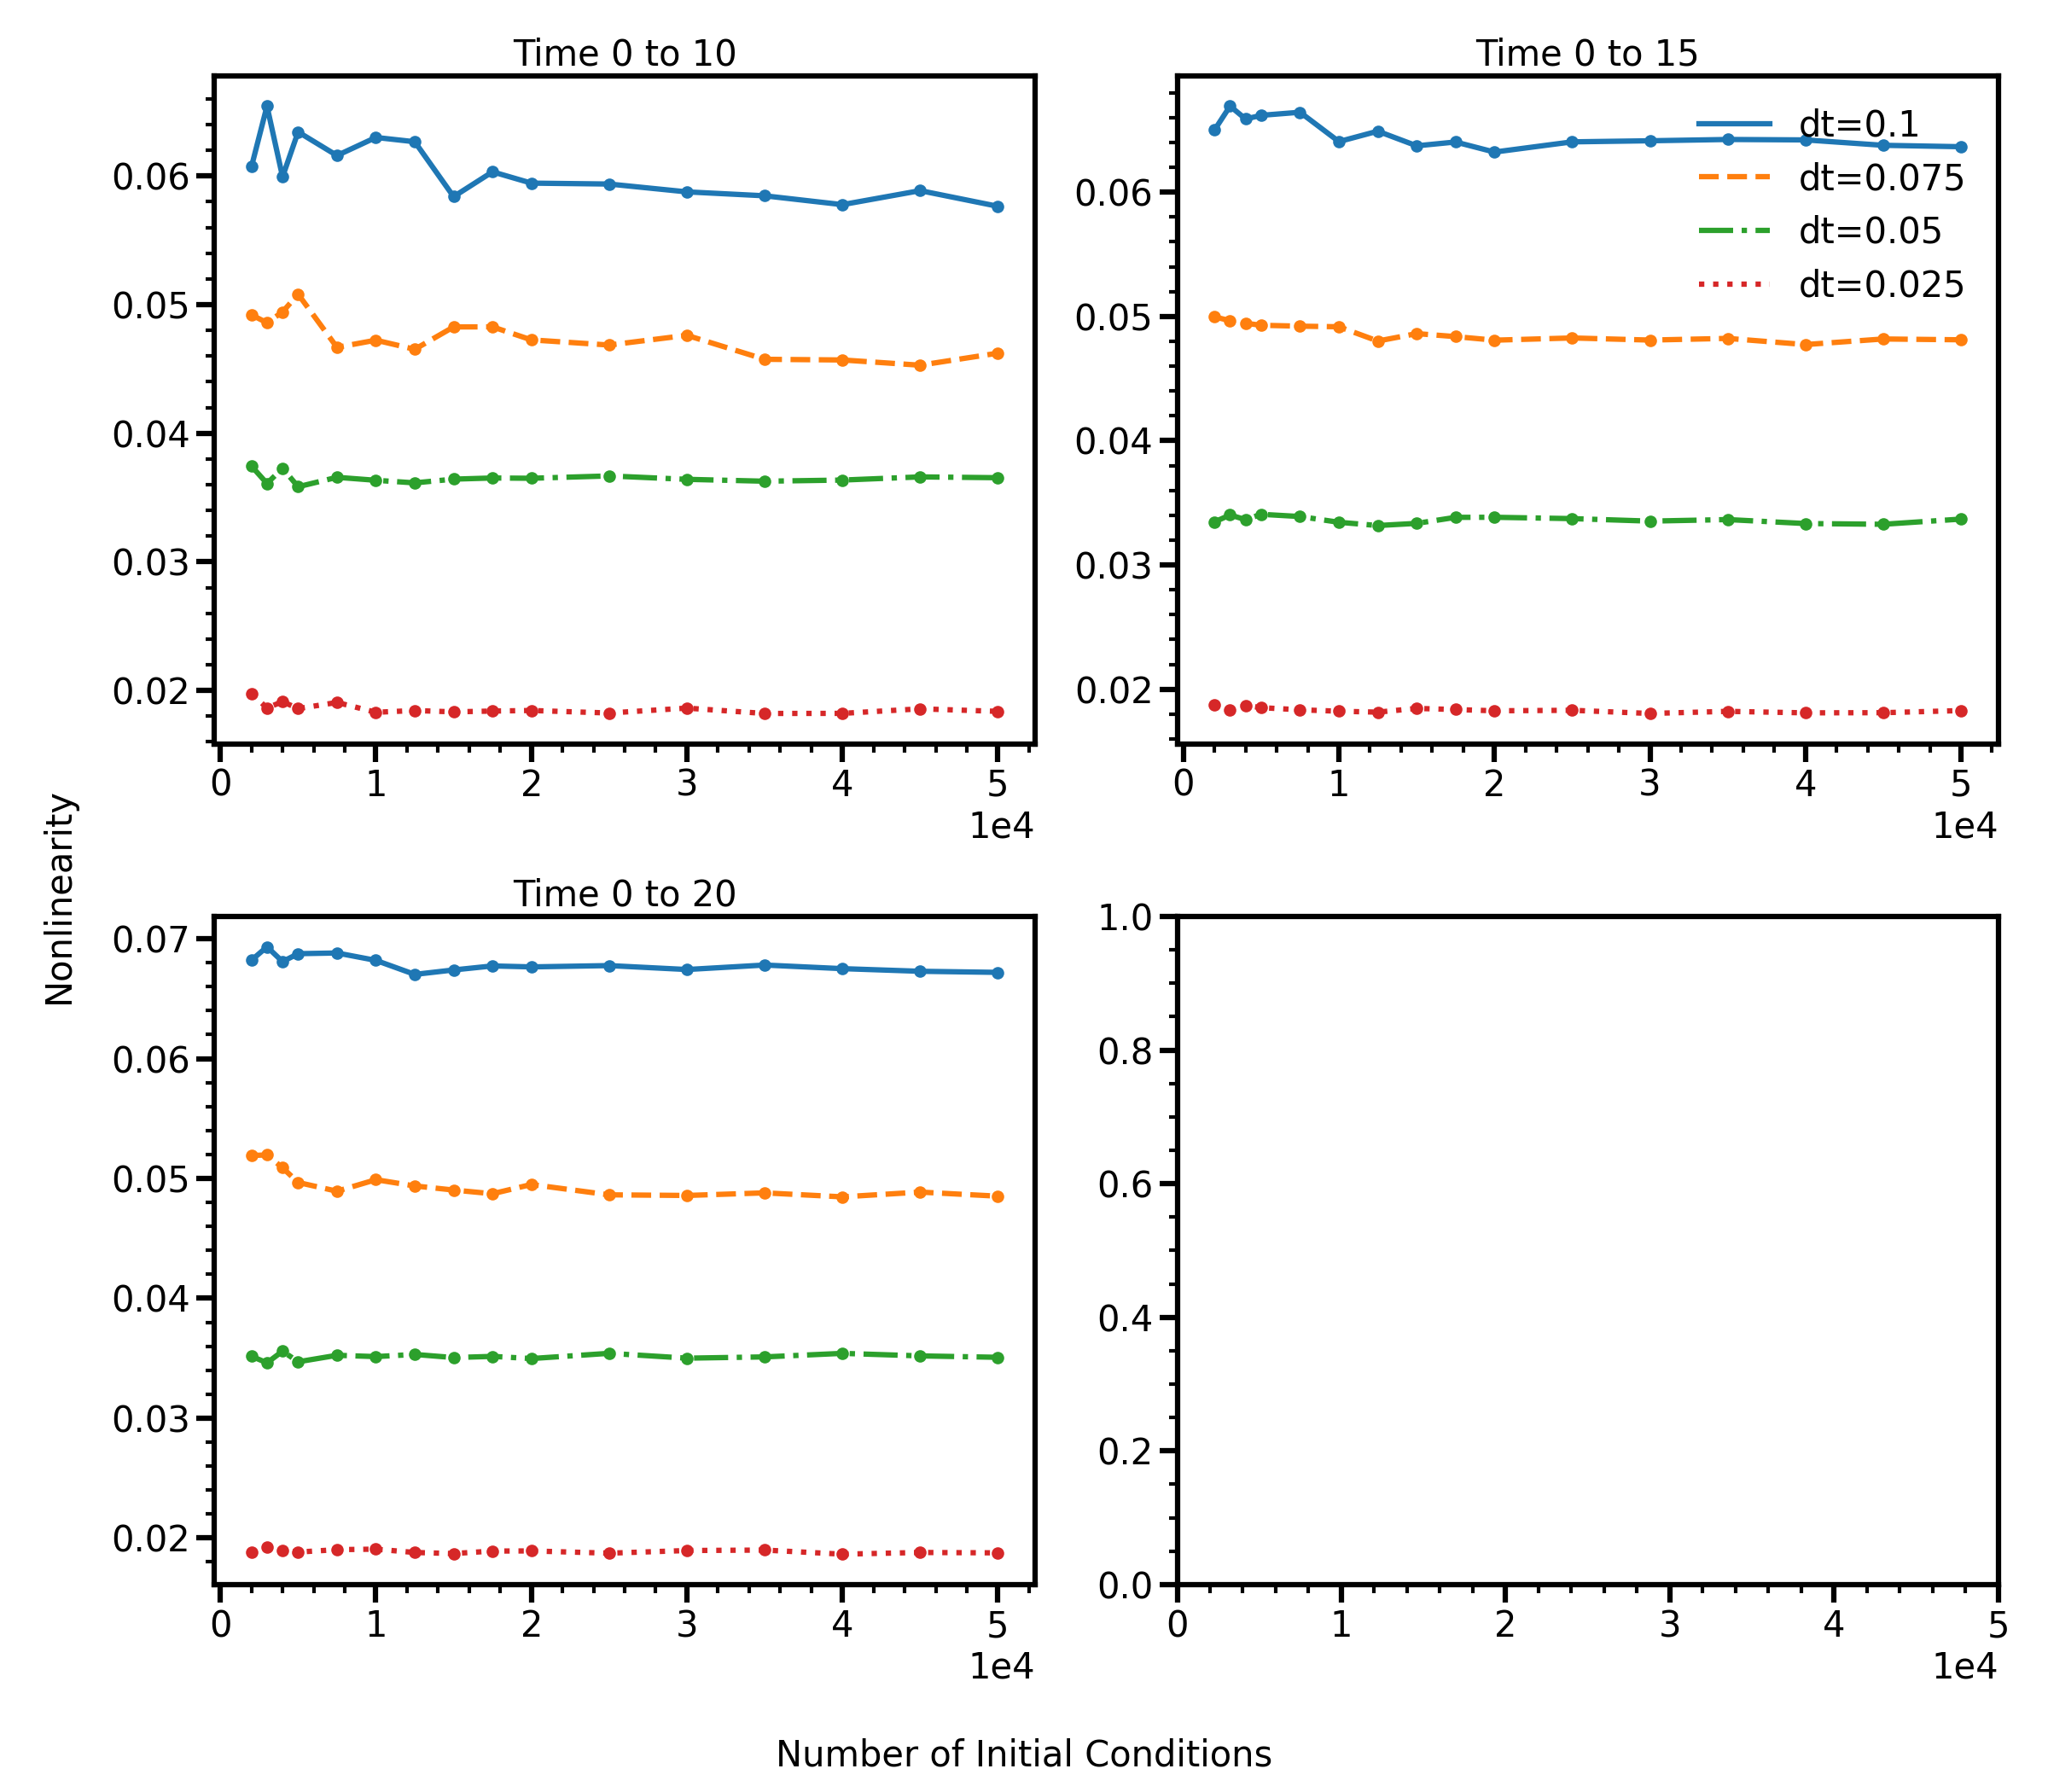
\includegraphics[width=\linewidth]{figures/nonnorm_nonlinearity}
	
	\caption{Nonlinearities before normalization.}\label{nonnorm_nonlinear}
\end{figure}

\begin{multicols}{2}

We may first note that the nonlinearity values are all decidedly nonzero and reasonably larger than the linear recovery values, indicating that our model is indeed nonlinear in the compressed space.  We also note the nonlinearity is much more erratic than the linear recovery.


\subsection{Accuracy}\label{Accuracy}
The primary accuracy metric which we have used is the validation loss normalized with the timestep.  This metric can essentially be interpreted as the expected L2 distance between the predicted evolution at time $t=1$ and the true evolution at $t=1$.  Smaller is better.

\end{multicols}

\begin{figure}
	\centering

	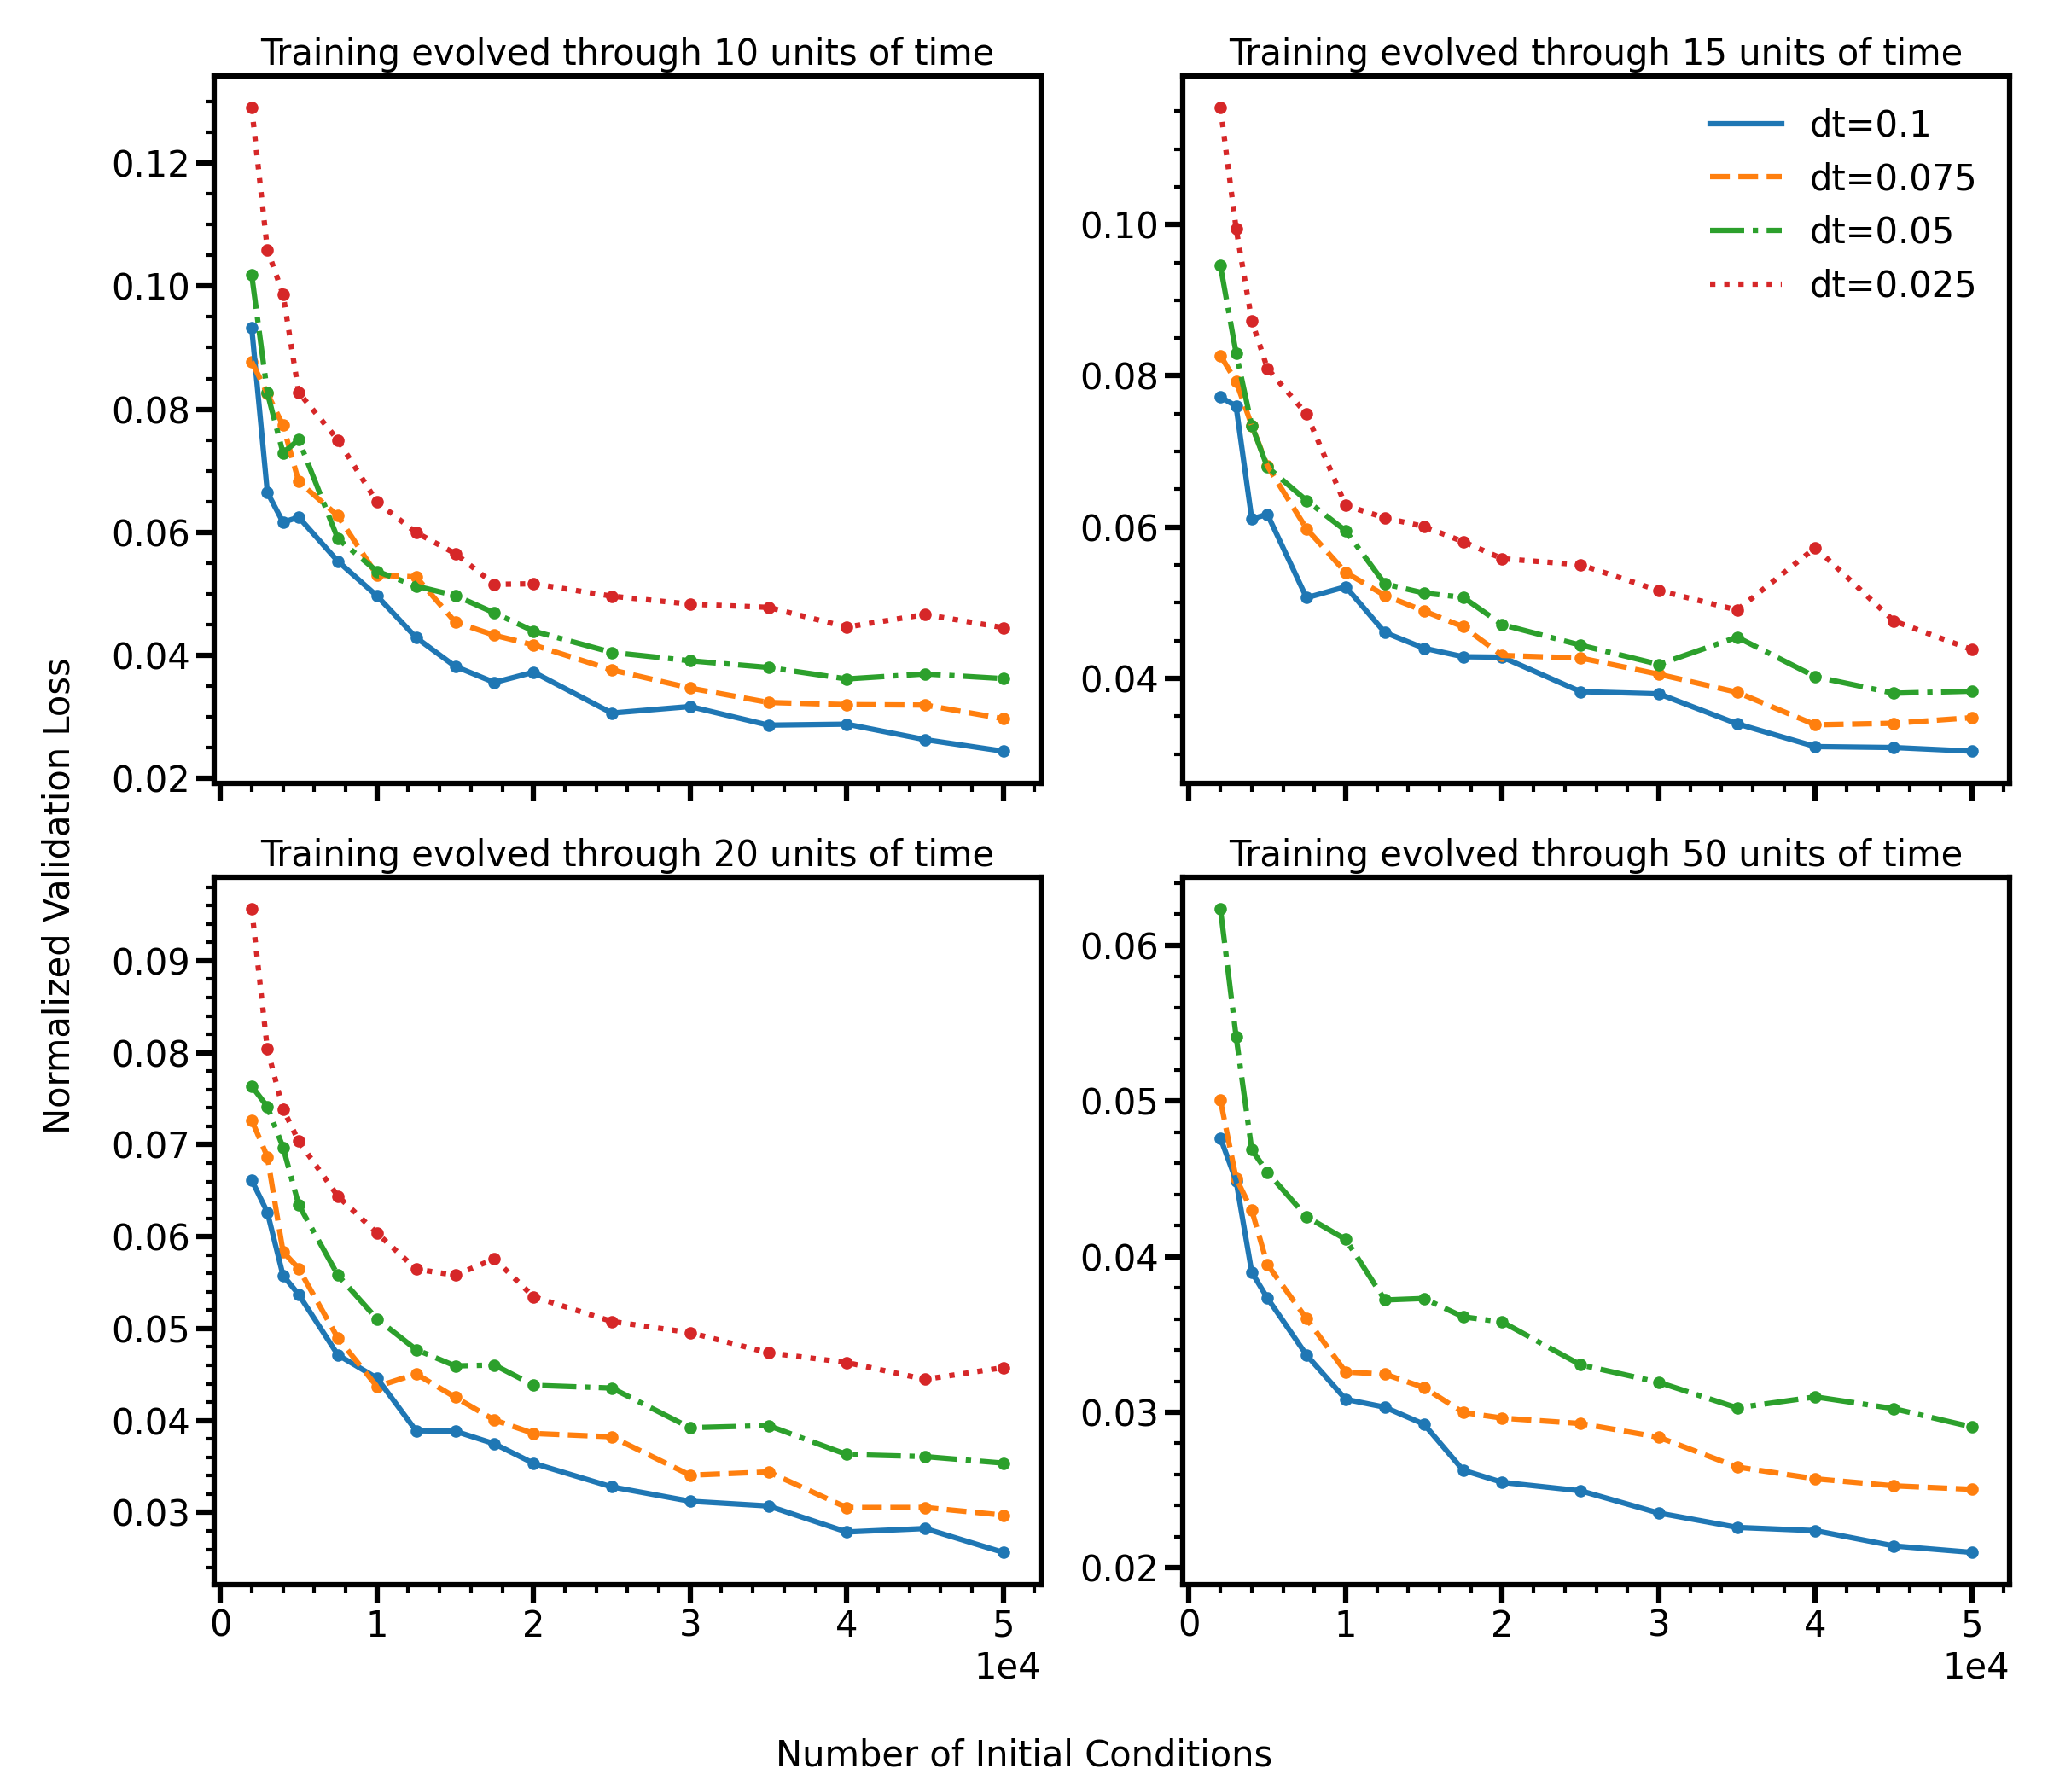
\includegraphics[width=\linewidth]{figures/norm_val_loss}

	\caption{Plots of the normalized validation loss.  Note the difference in scale of each plot.}\label{norm_val_loss}

\end{figure}

\begin{figure}
	\centering
	
	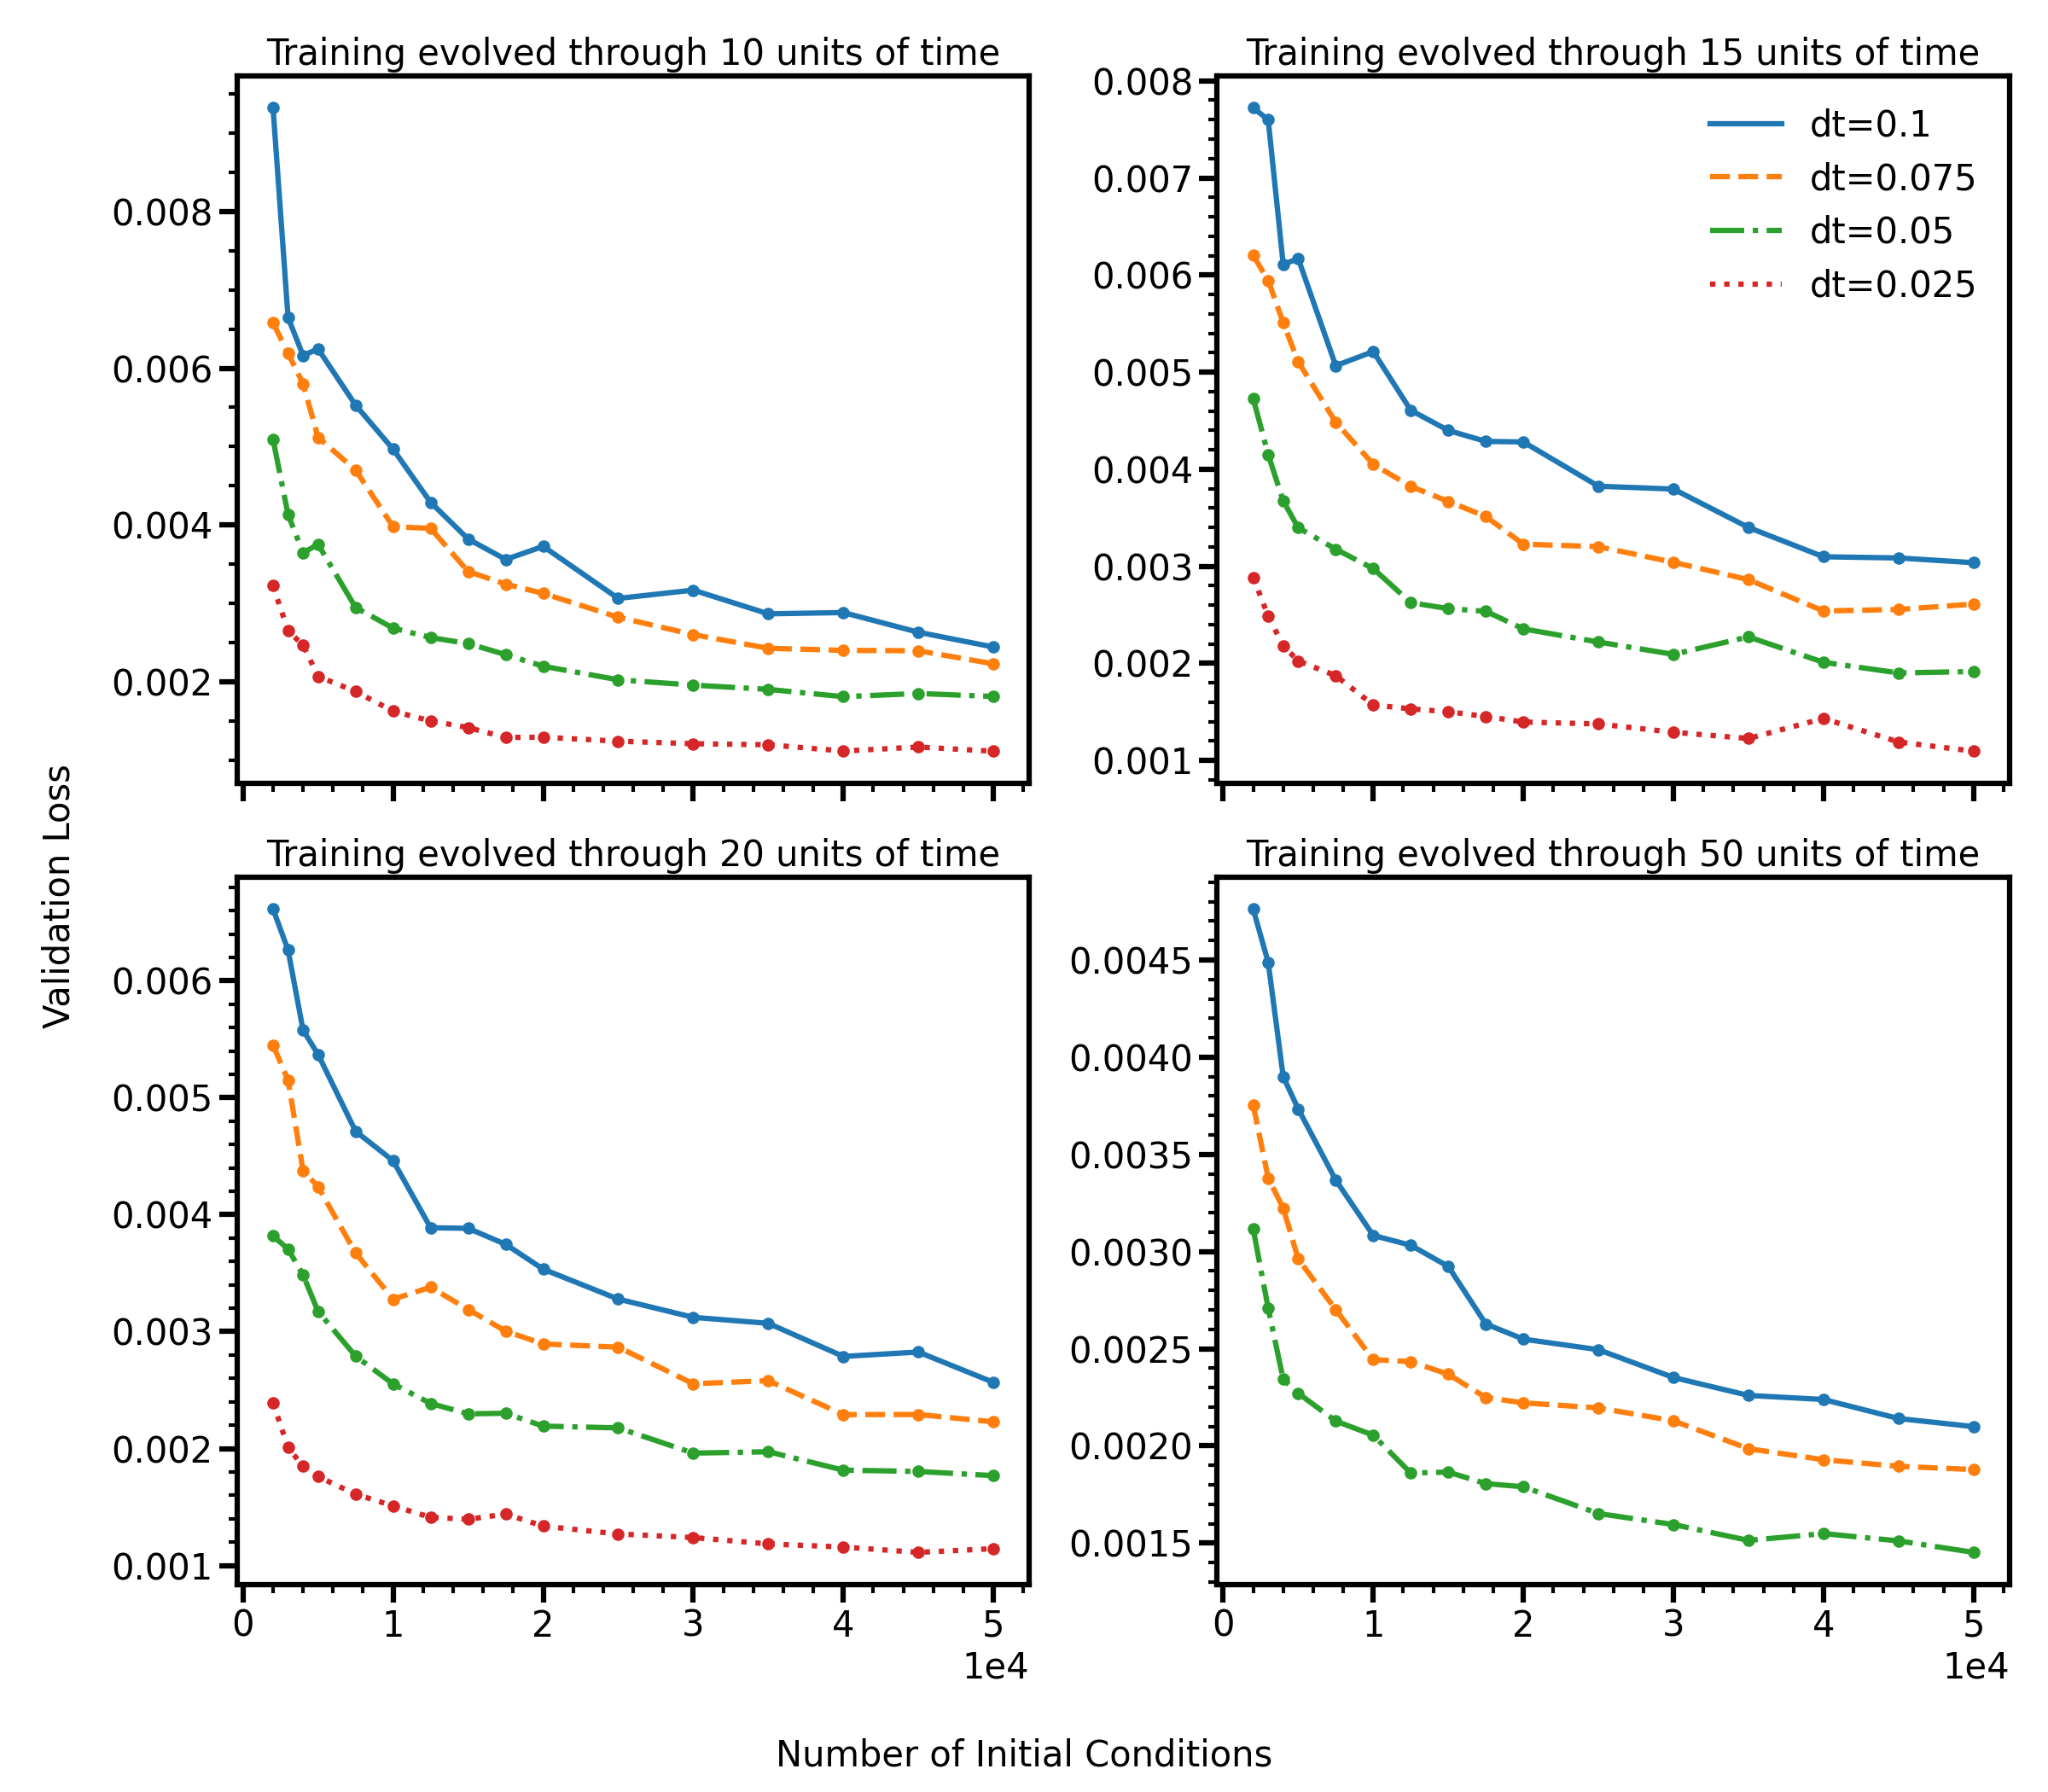
\includegraphics[width=\linewidth]{figures/nonnorm_val_loss}
	\caption{Validation loss before normalization.  Note that all values are below $10^{-2}$, indicating that the model is accurate to two decimals step-to-step.}\label{nonnorm_val_loss}
\end{figure}

\begin{multicols}{2}

We note that upon normalization, shorter timesteps lead to a larger overall error despite the smaller local error.  This implies that while the local error does decrease with the timestep as we would expect, it does not decrease as quickly as the number of timesteps required to evolve the same amount of time increases.  As expected, evolving the system for longer yields better accuracy both globally and locally.  We note however that this is not due simply to an increase in the number of training points; the system evolved for 10 units of time with a timestep of 0.05 has the same number of points as the system evolved for 20 units of time with a timestep of 0.1, yet the latter system preforms better.  

As we would expect, the accuracy of our model increases as we give it more initial conditions to train on.  We believe that there is a plateau beginning to form around 40000 initial conditions, however. 

\end{multicols}

\newpage

\appendix

\section{Additional Plots}

\begin{figure}
	\centering
	
	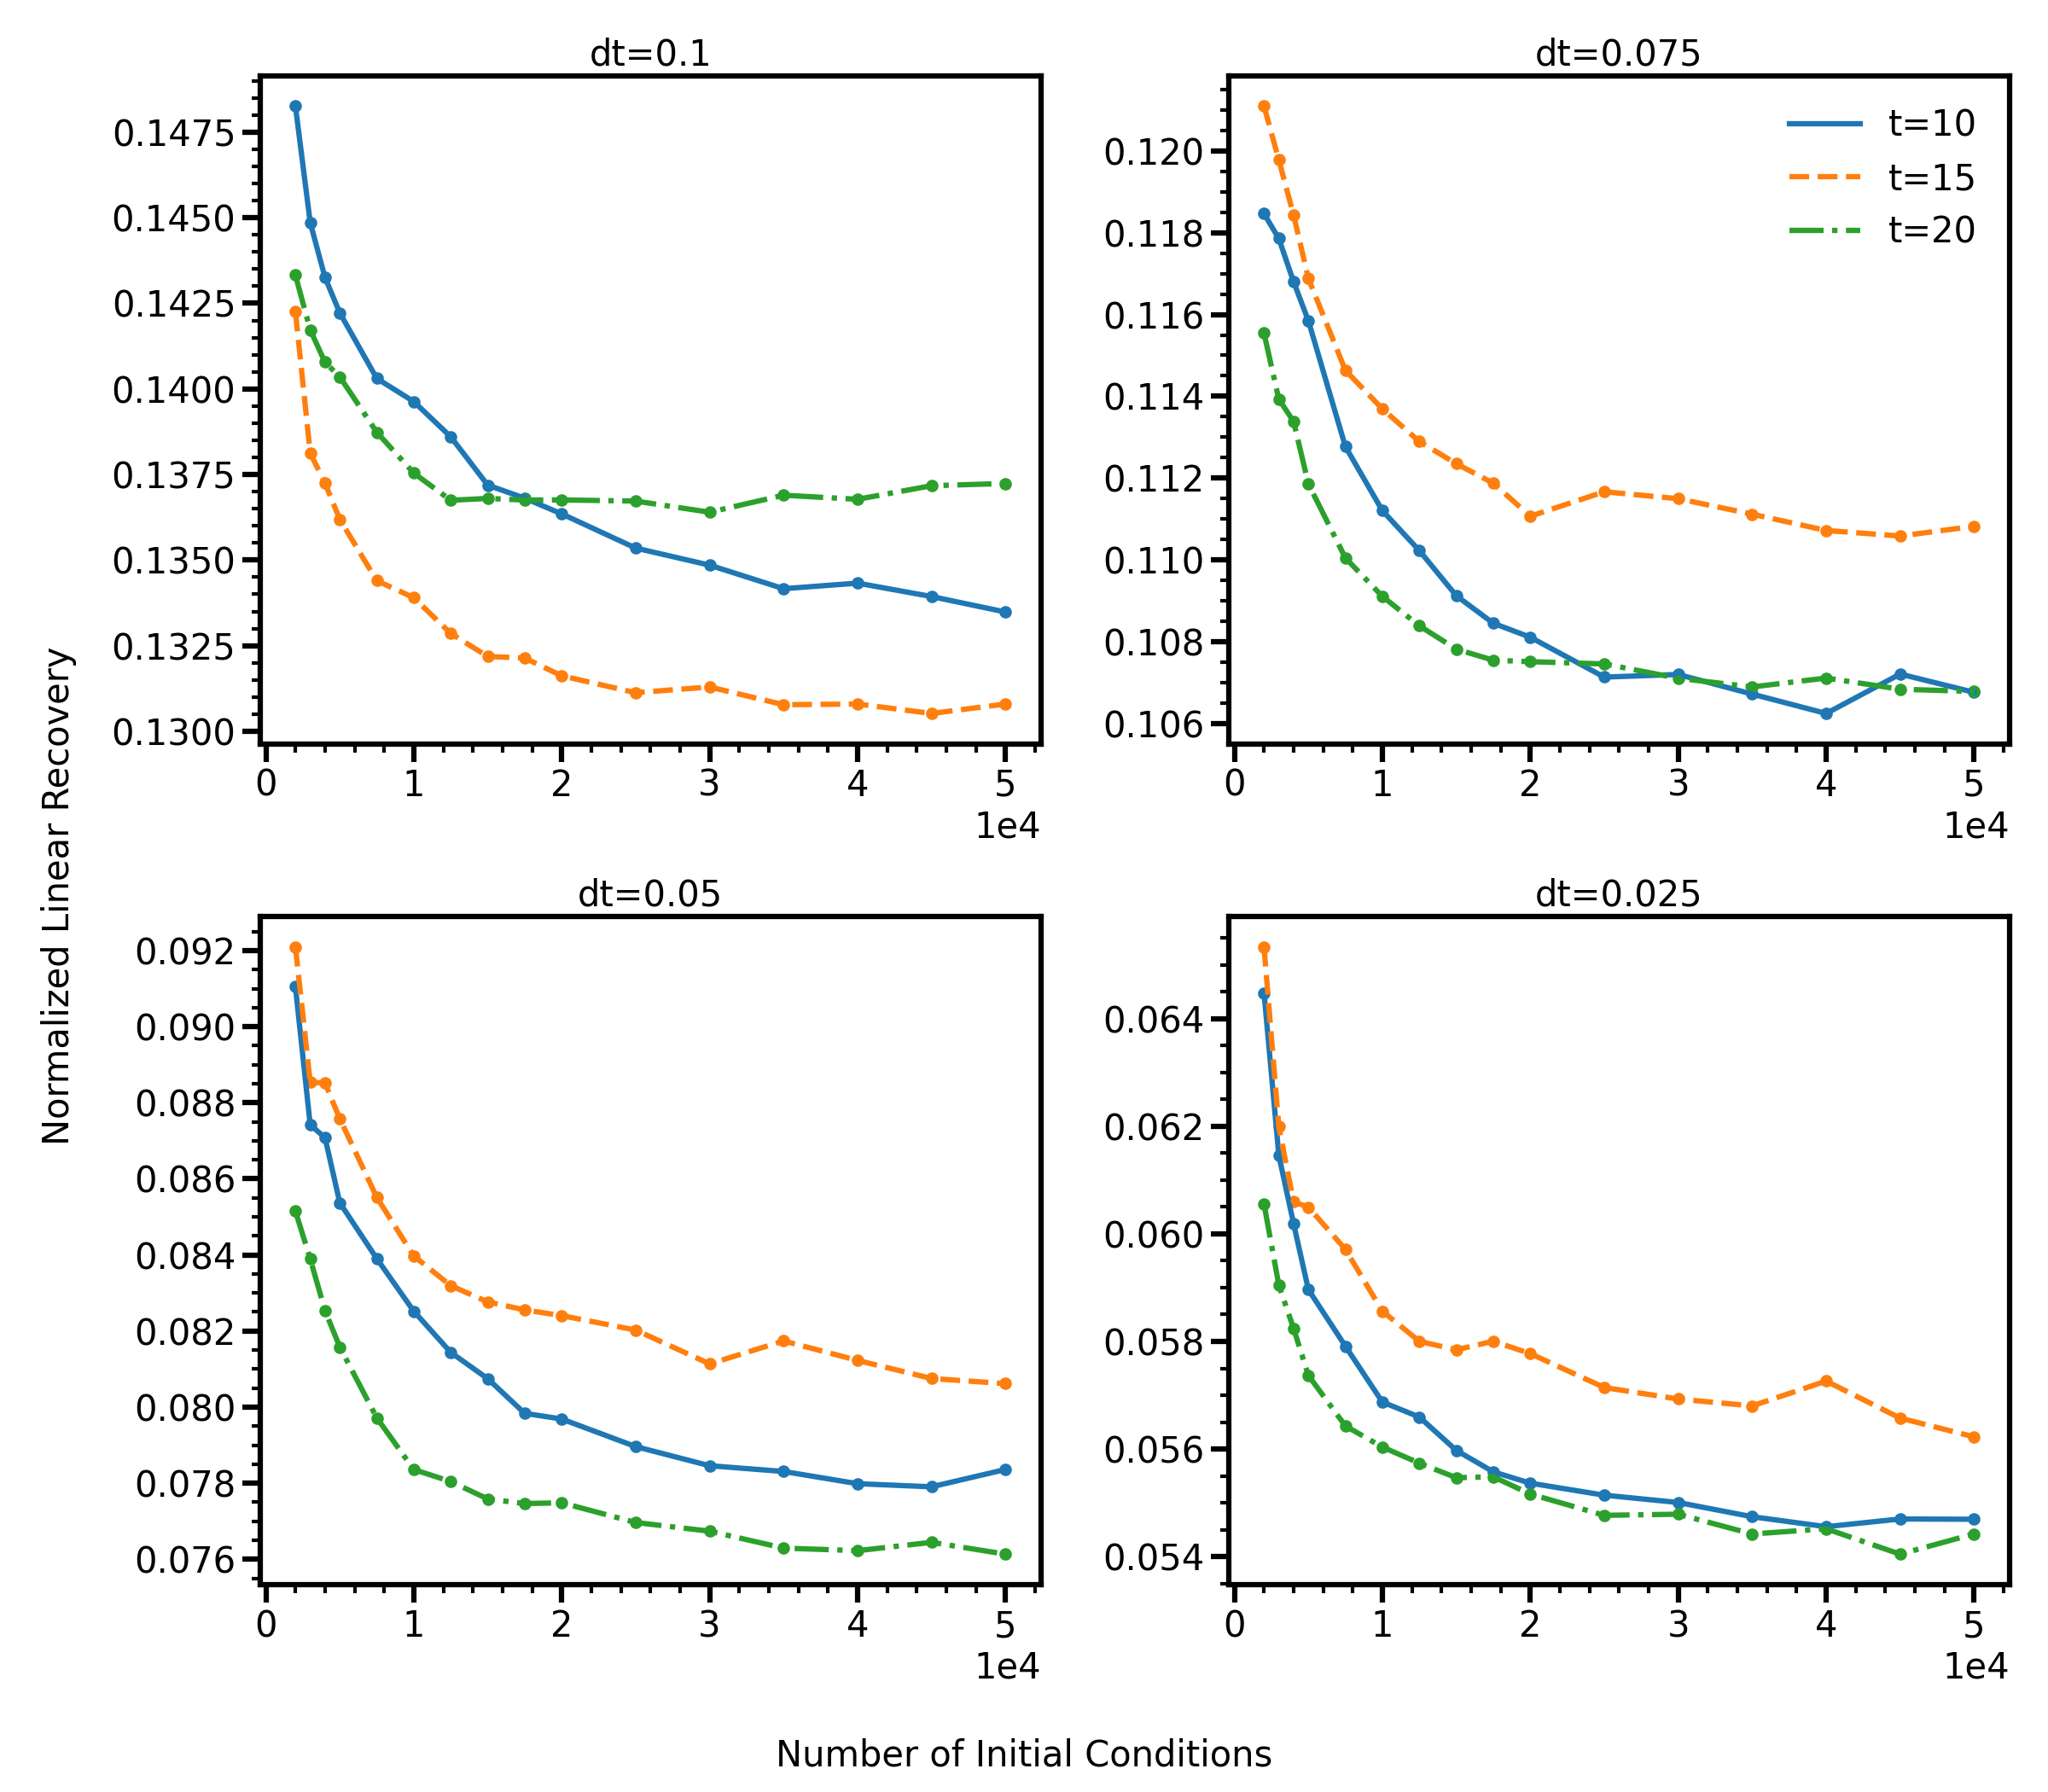
\includegraphics[width=\linewidth]{figures/norm_linear_recovery_evolve_time}
	\caption{Normalized linear recovery, now with each plot having a constant timestep rather than a constant evolve time as in figure \ref{norm_linear_recovery}}\label{norm_linear_recovery_evolve_time}
\end{figure}

\begin{figure}
	\centering
	
	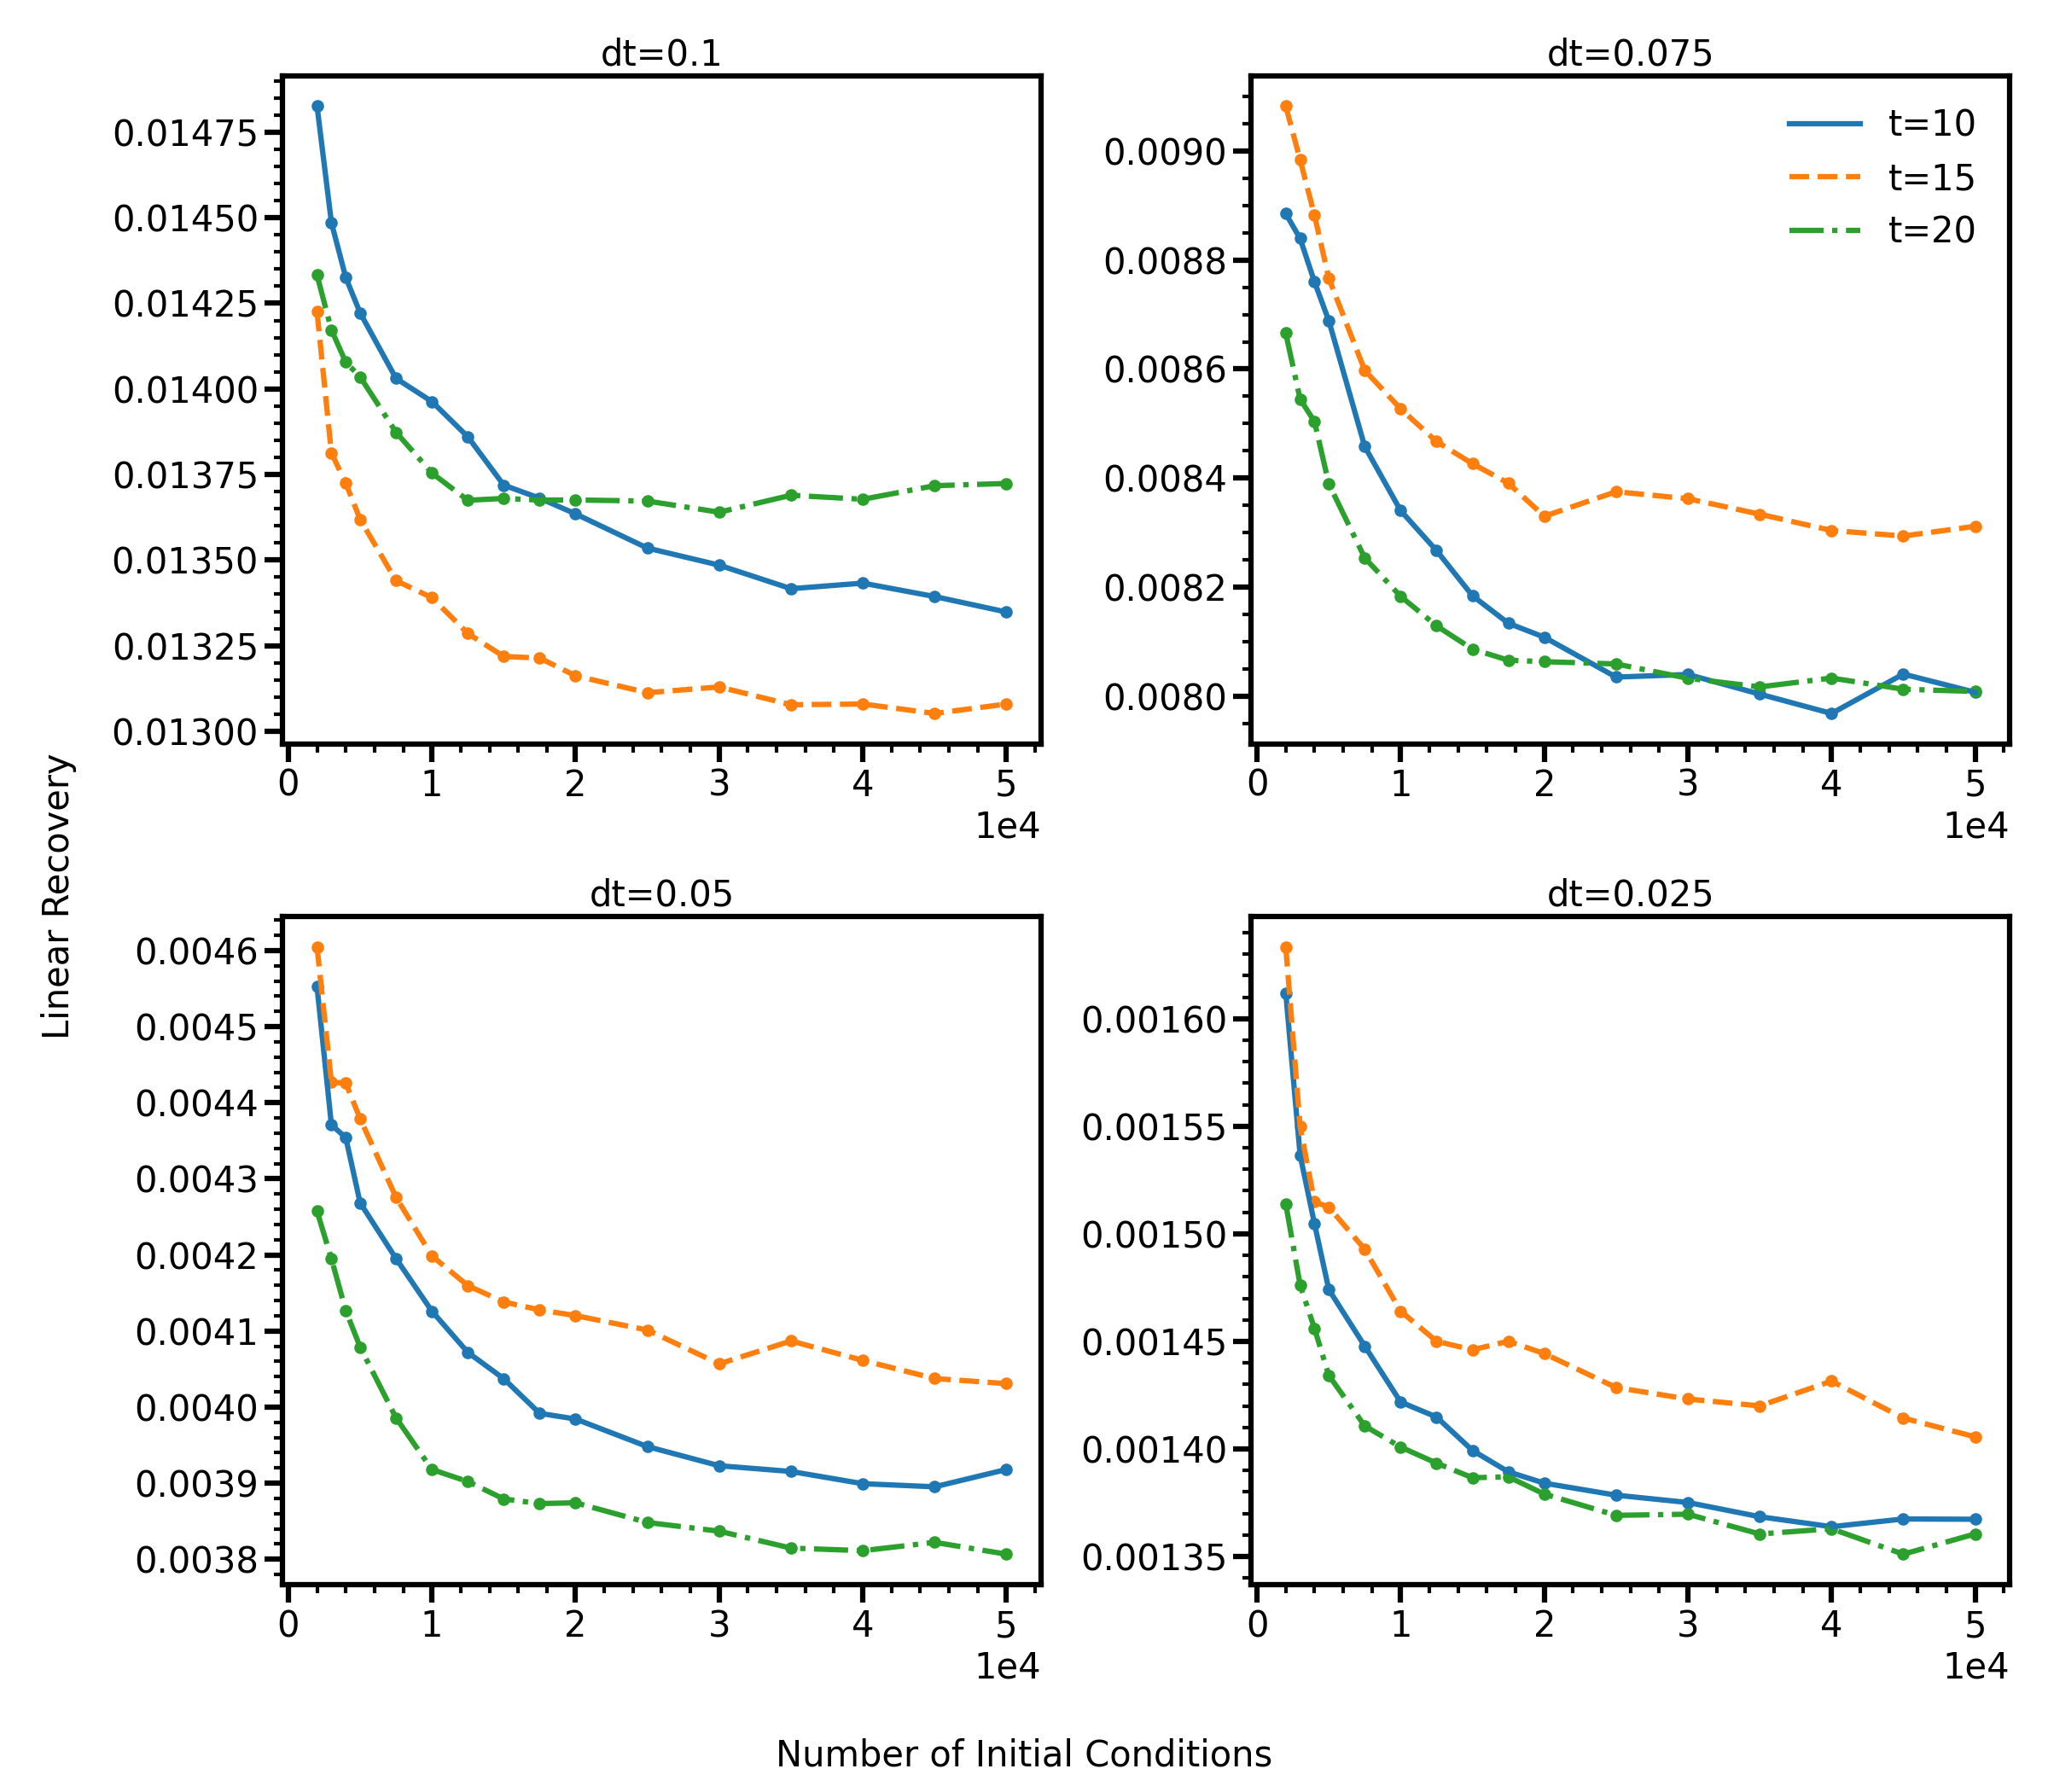
\includegraphics[width=\linewidth]{figures/nonnorm_linear_recovery_evolve_time}
	\caption{Non-normalized linear recovery, now with each plot having a constant timestep rather than a constant evolve time as in figure \ref{nonnorm_linear_recovery}}\label{nonnorm_linear_recovery_evolve_time}
\end{figure}

\begin{figure}
	\centering
	
	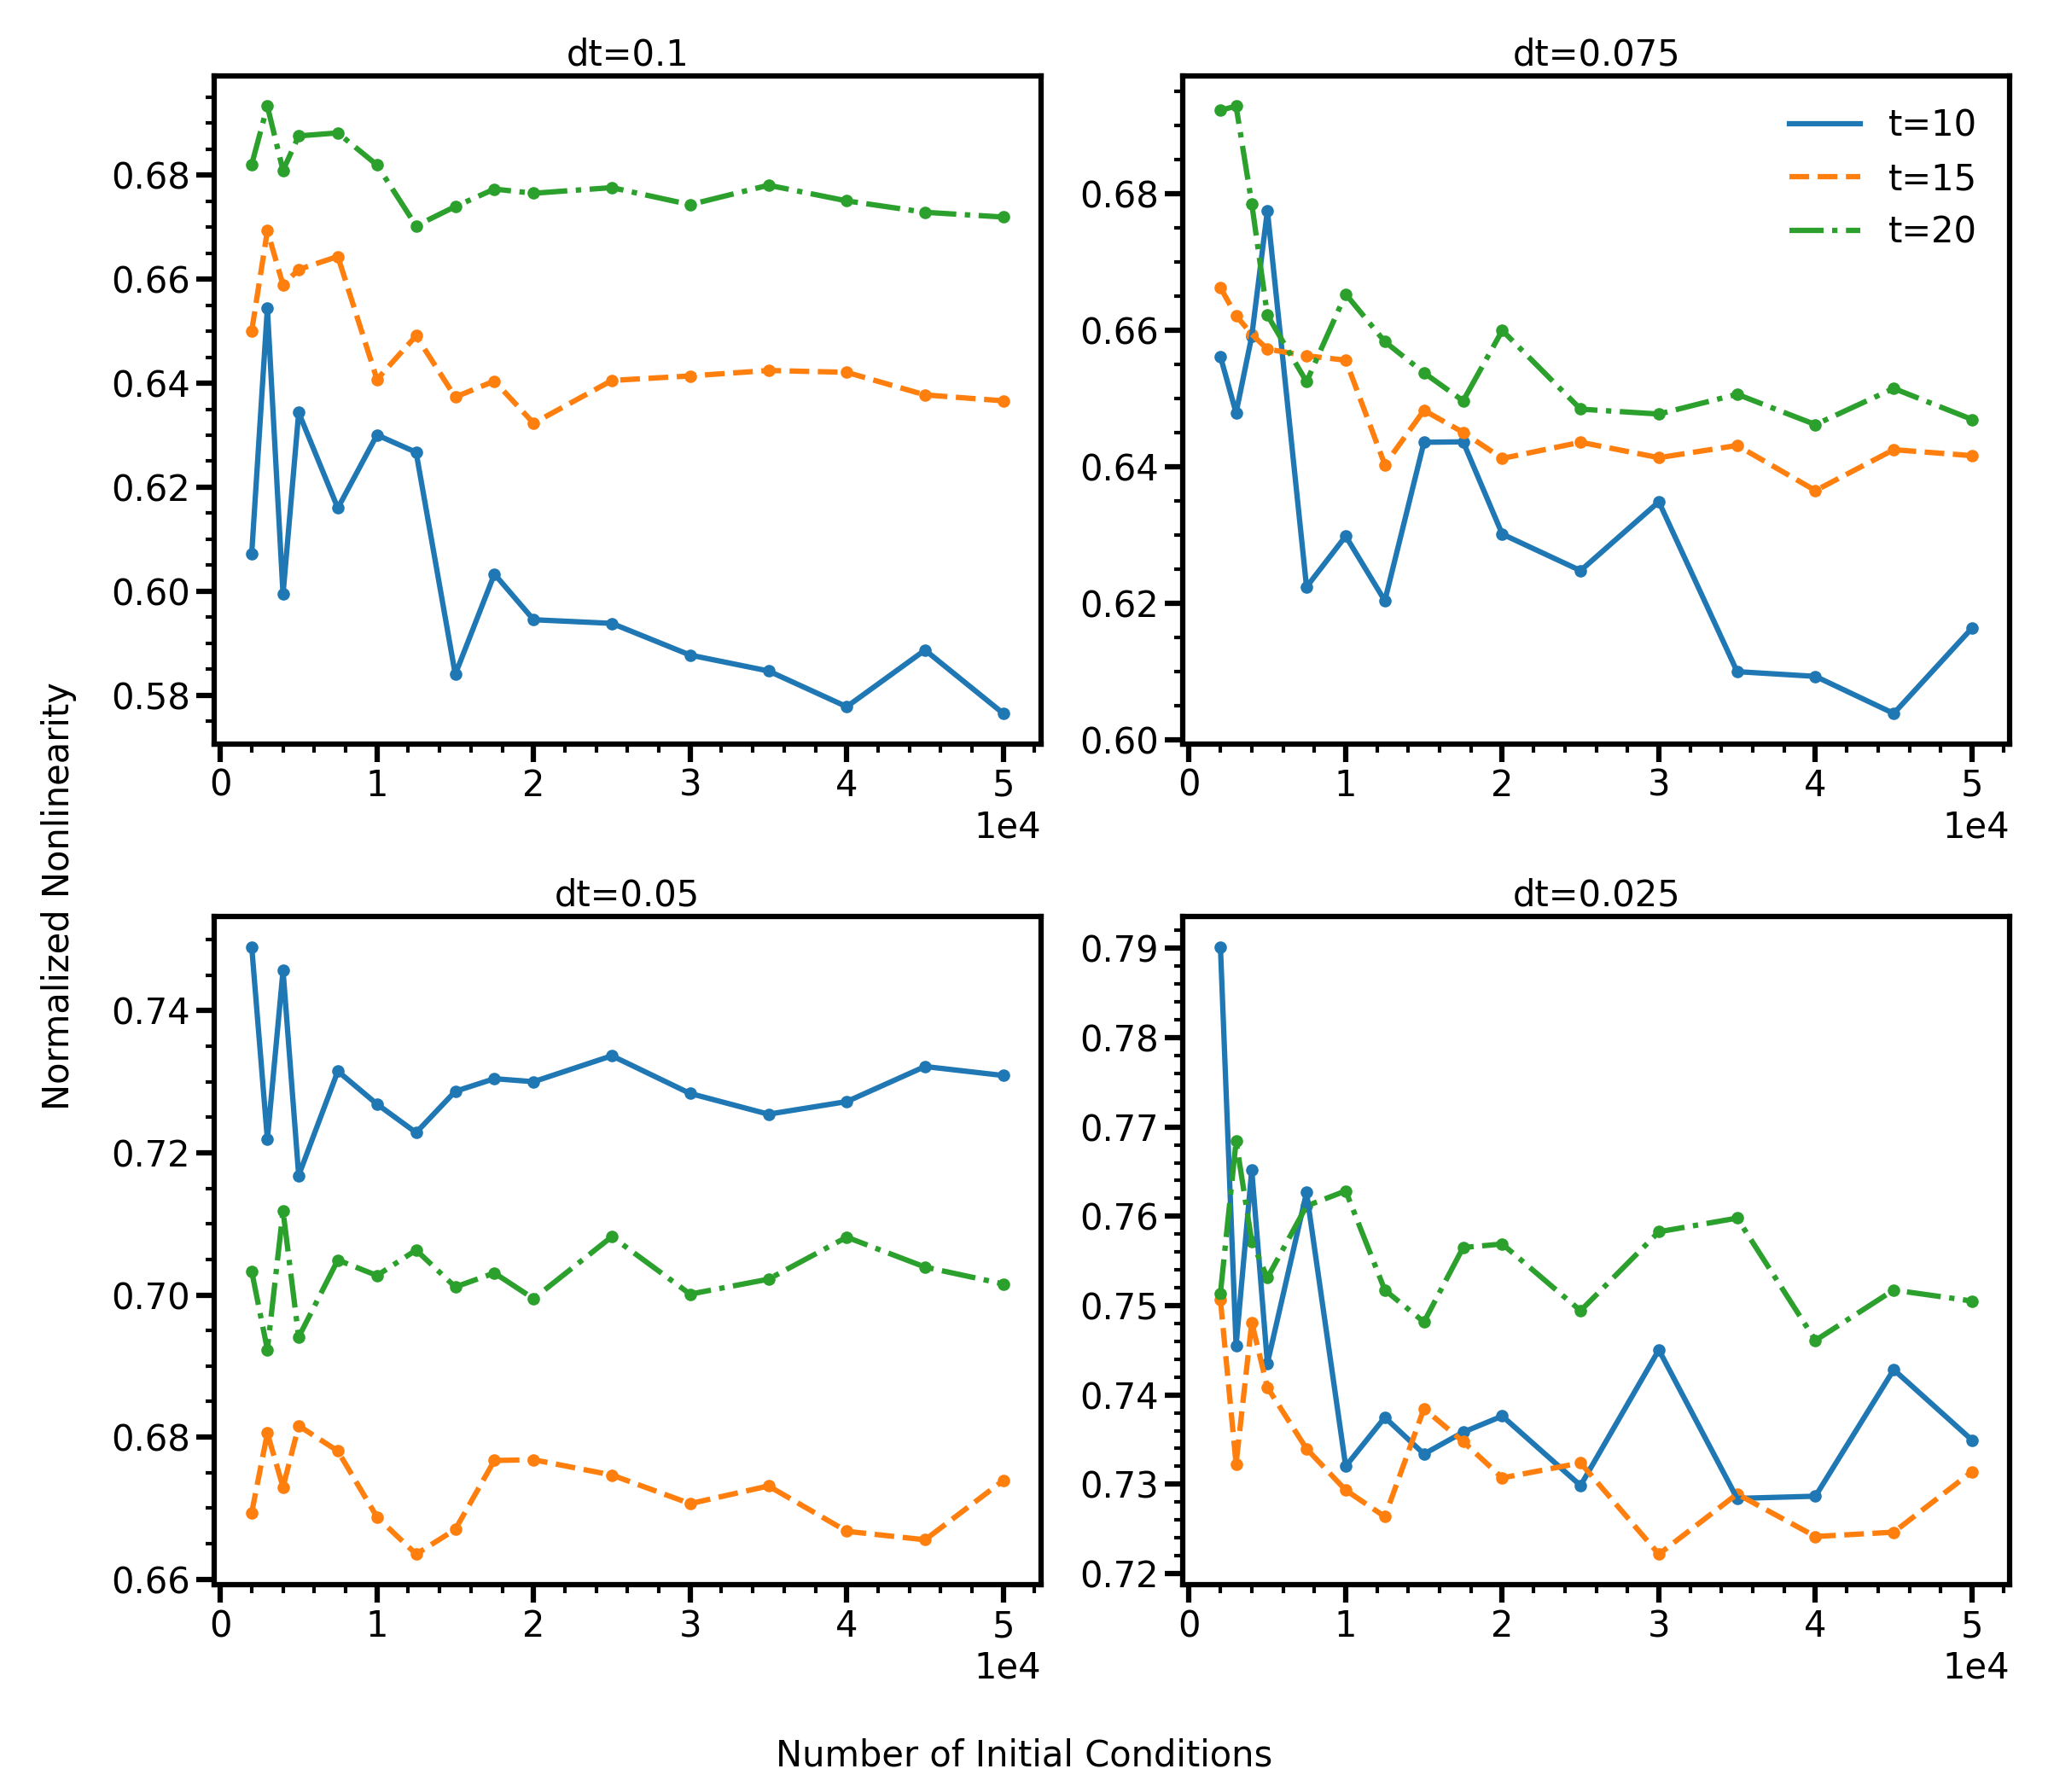
\includegraphics[width=\linewidth]{figures/norm_nonlinearity_evolve_time}
	\caption{Normalized nonlinearity, now with each plot having a constant timestep rather than a constant evolve time as in figure \ref{norm_nonlniear}}\label{norm_nonlinear_evolve_time}
\end{figure}

\begin{figure}
	\centering
	
	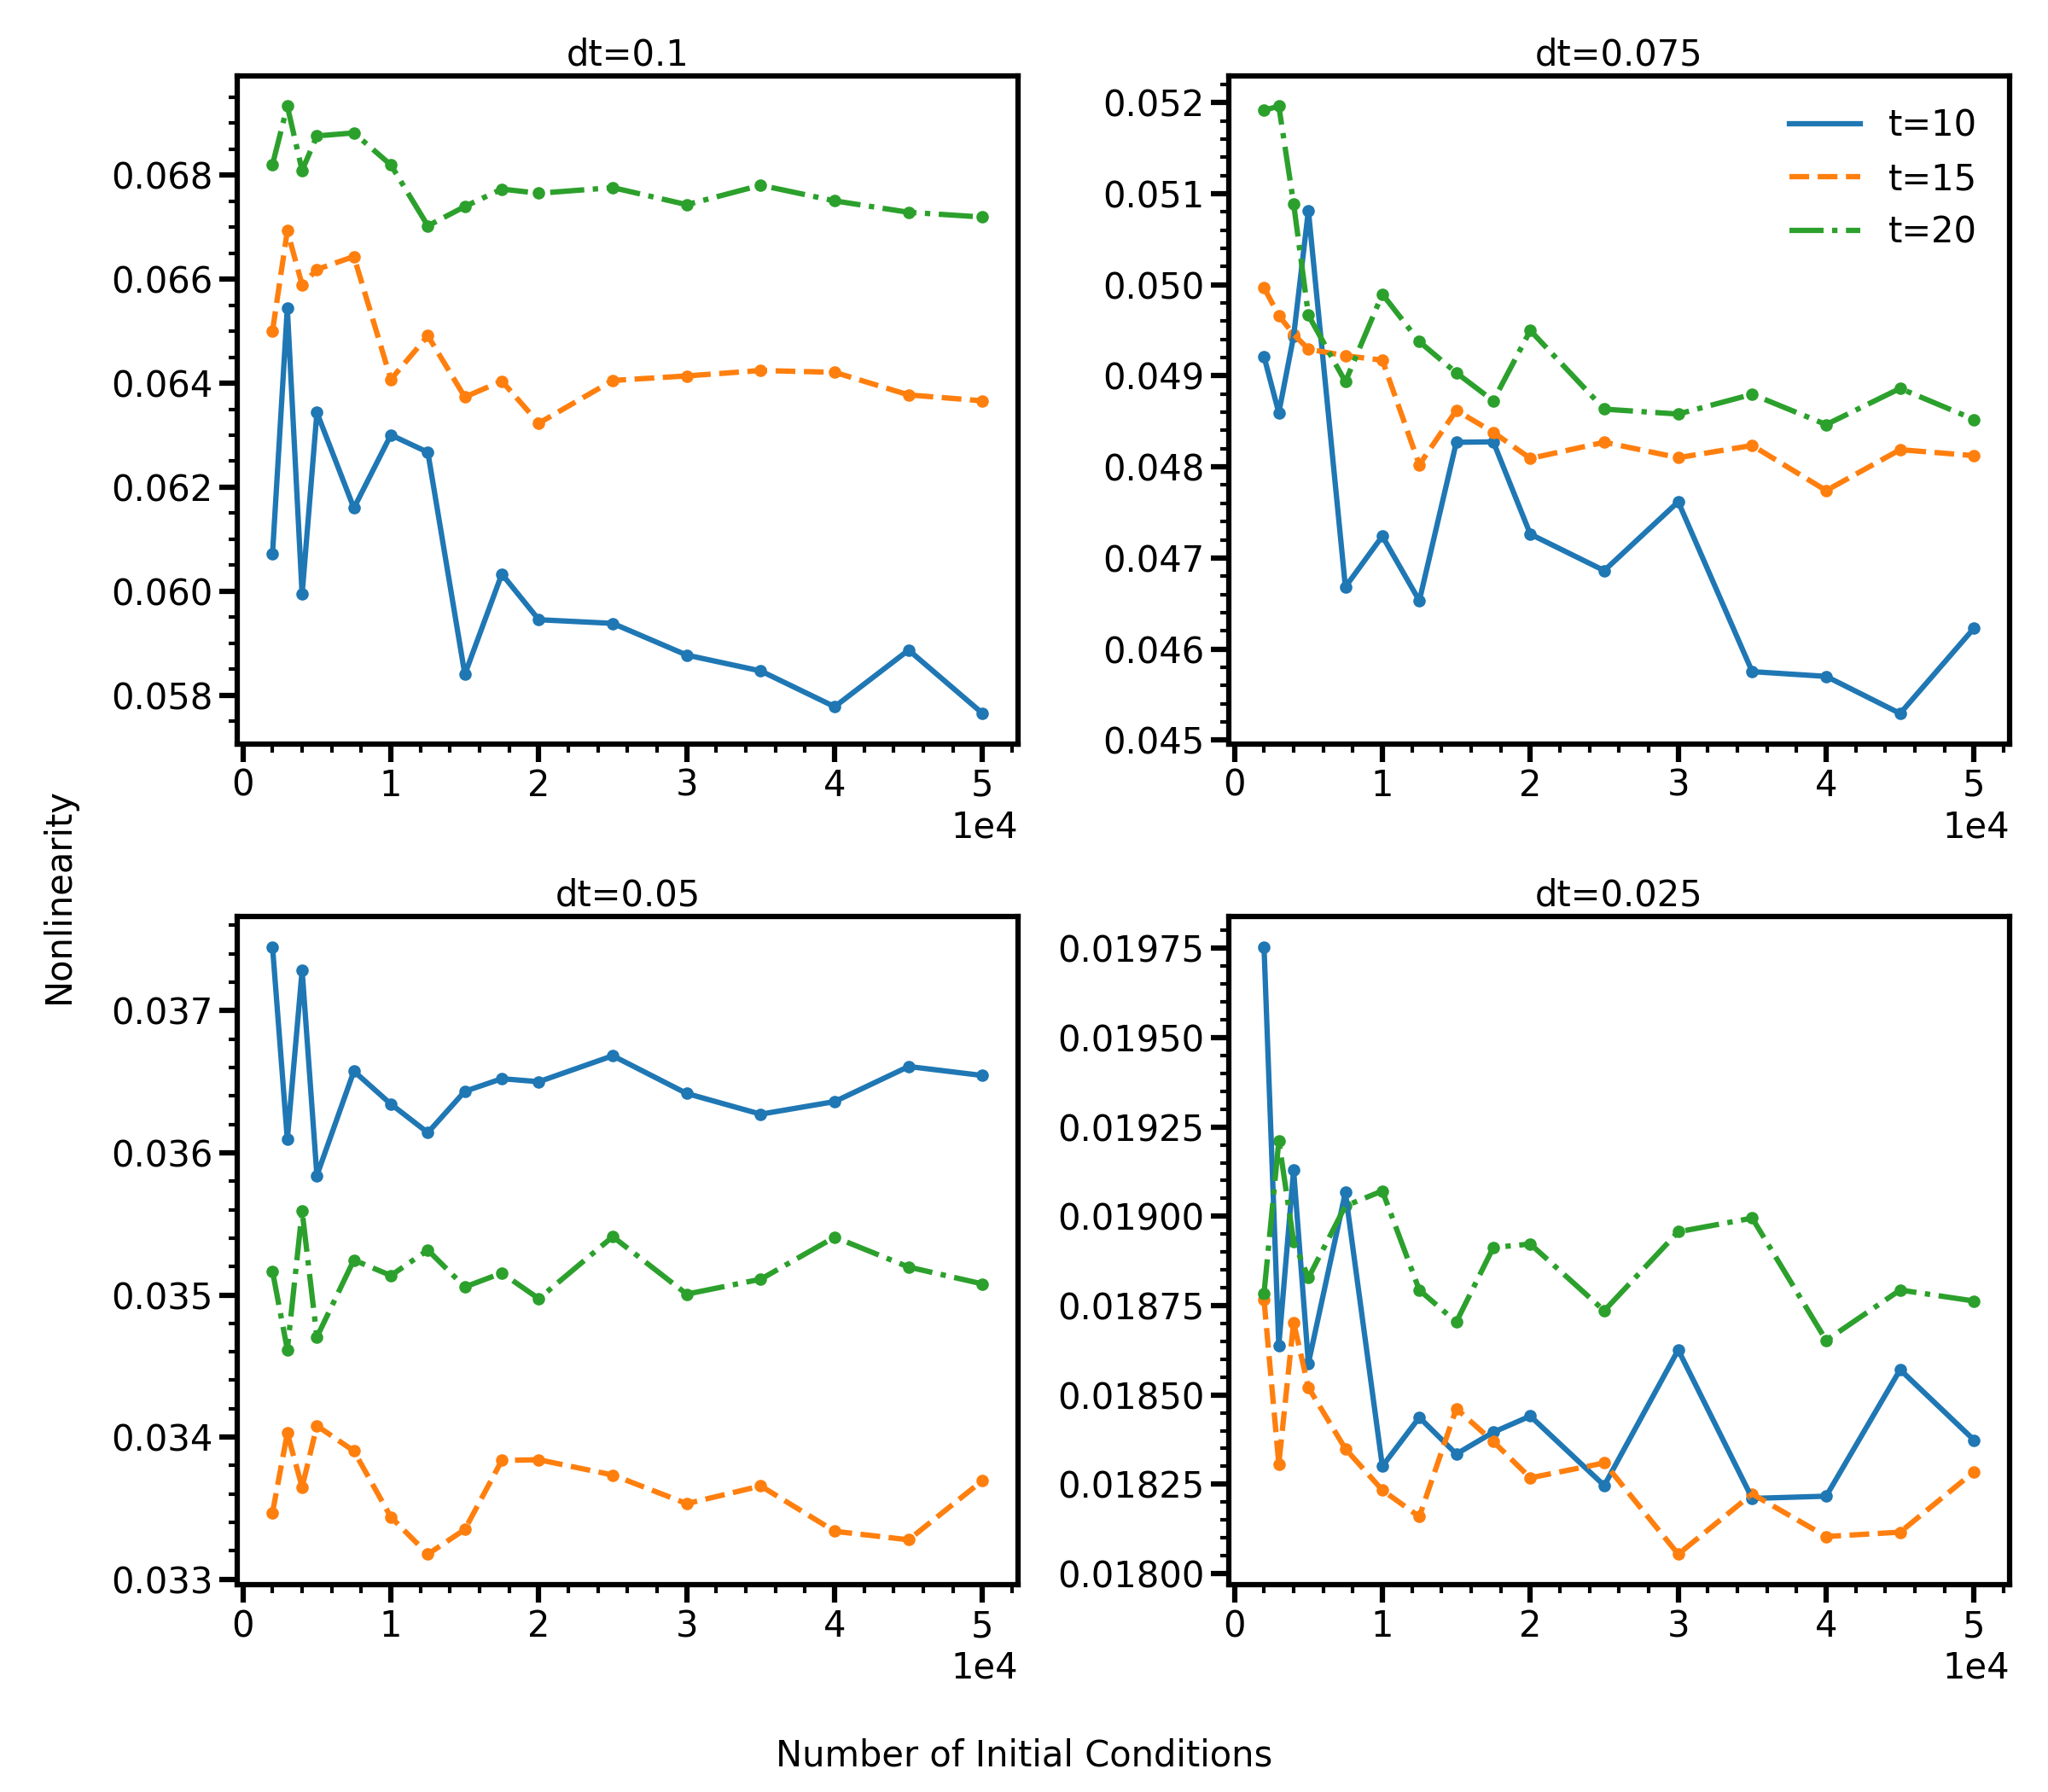
\includegraphics[width=\linewidth]{figures/nonnorm_nonlinearity_evolve_time}
	\caption{Normalized nonlinearity, now with each plot having a constant timestep rather than a constant evolve time as in figure \ref{nonnorm_nonlniear}}\label{nonnorm_nonlinear_evolve_time}
\end{figure}

\begin{figure}
	\centering
	
	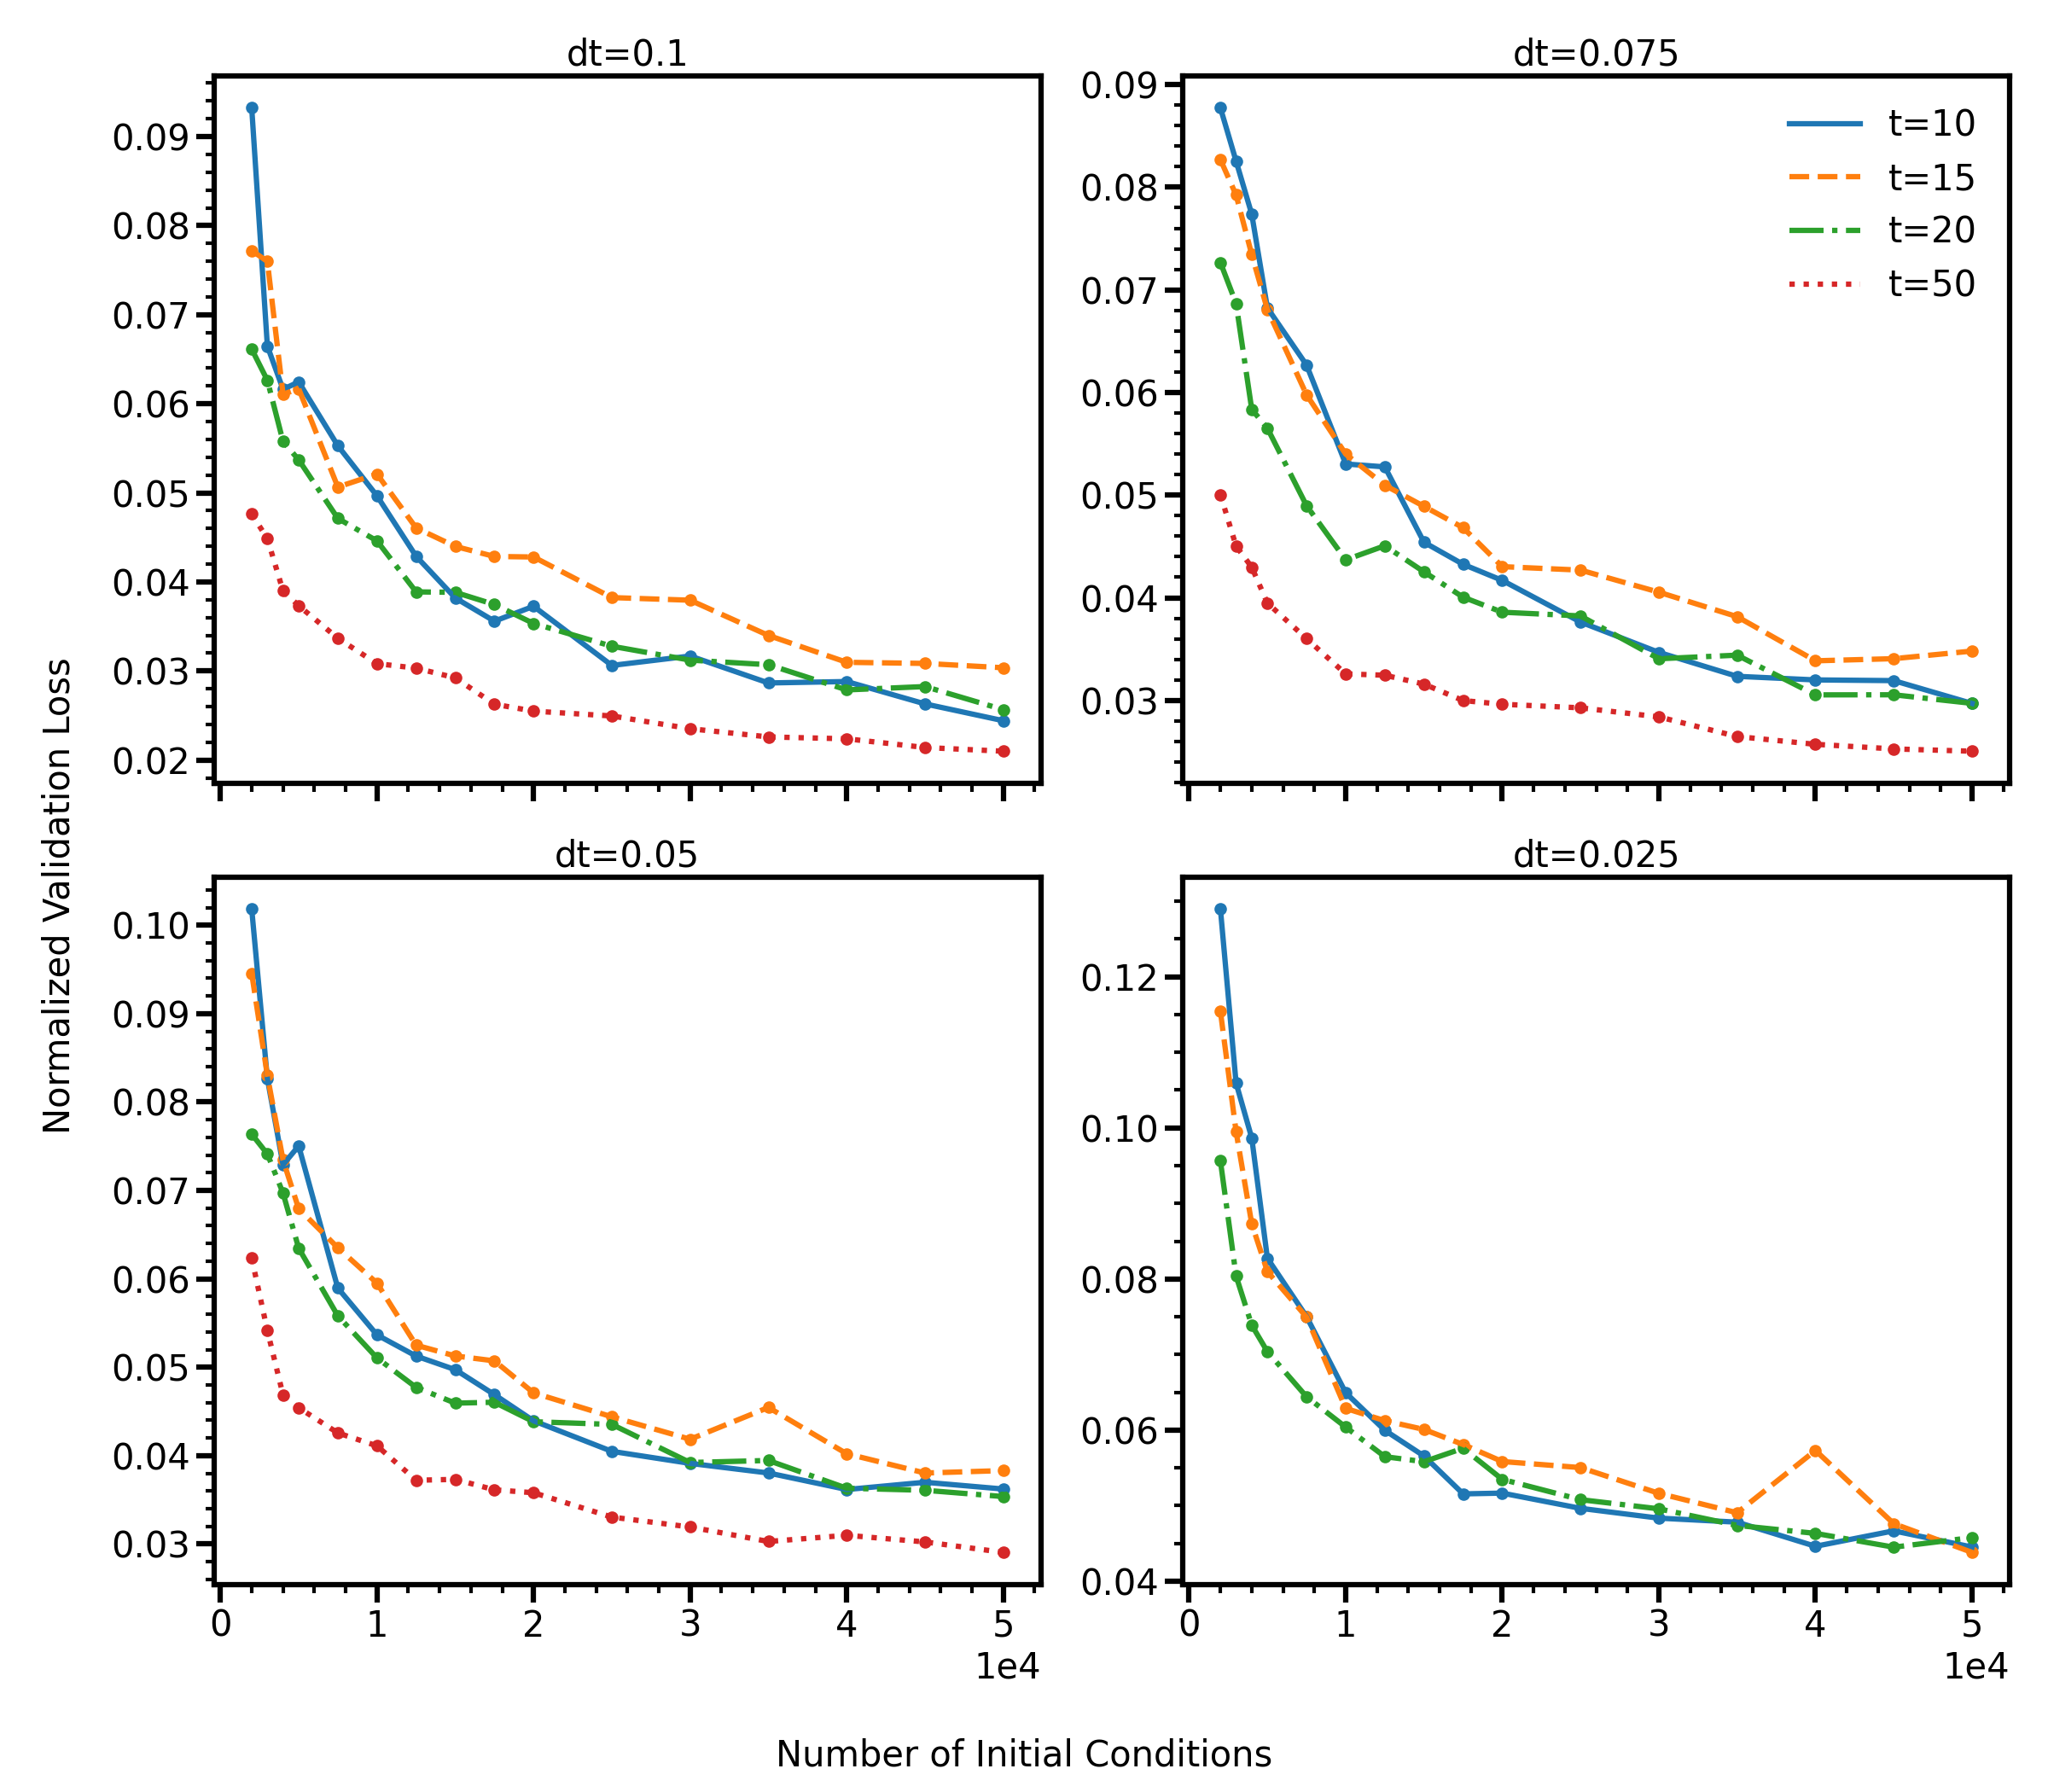
\includegraphics[width=\linewidth]{figures/norm_val_loss_evolve_time}
	\caption{Normalized nonlinearity, now with each plot having a constant timestep rather than a constant evolve time as in figure \ref{norm_val_loss}}\label{norm_val_loss_evolve_time}
\end{figure}

\begin{figure}
	\centering
	
	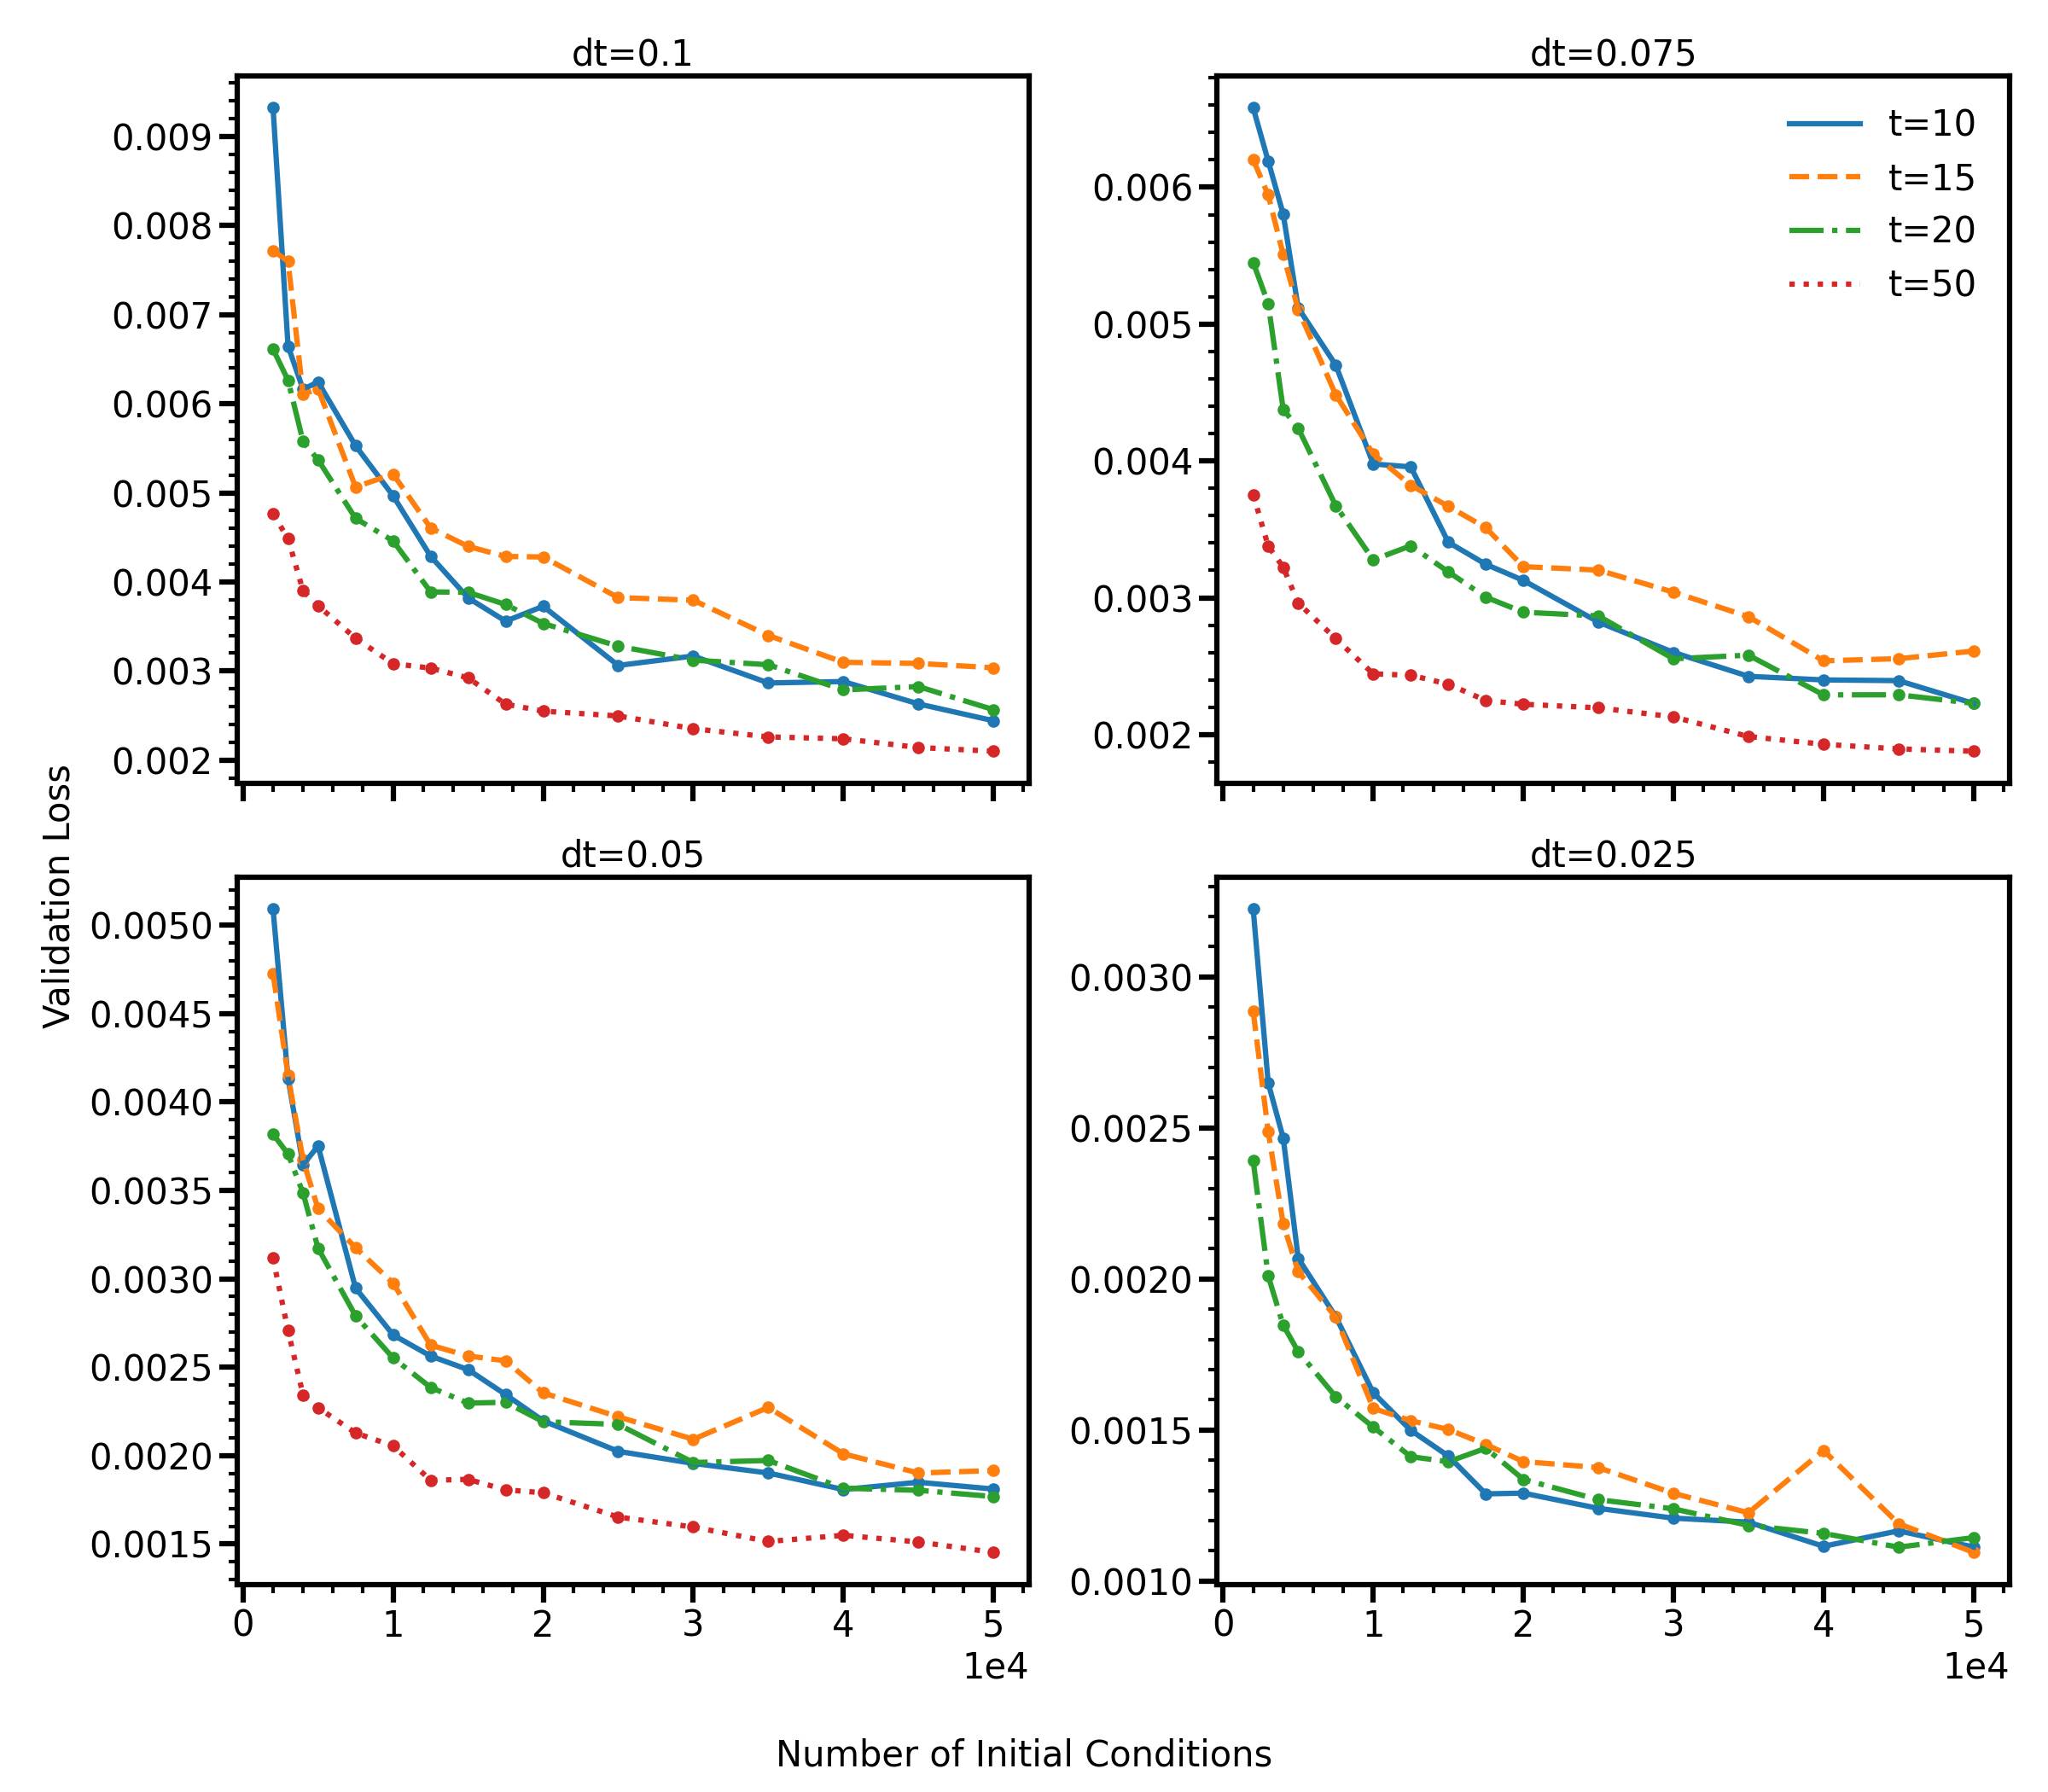
\includegraphics[width=\linewidth]{figures/nonnorm_val_loss_evolve_time}
	\caption{Normalized nonlinearity, now with each plot having a constant timestep rather than a constant evolve time as in figure \ref{nonnorm_val_loss}}\label{nonnorm_val_loss_evolve_time}
\end{figure}

%Plots with each plot constant on the dt axis rather than evolution time axis

%Example plots of the dynamics/true state of the system with a prediction overlain



\end{document}
